\documentclass[11pt]{article}
\usepackage[margin=1in]{geometry}
\usepackage{amsmath,amssymb,graphicx,booktabs,hyperref}
\graphicspath{{../results/figures/}}
\title{Inside the Swarm: Causal Mechanistic Interpretability of Emergent Collective Decision-Making in Neural Multi-Agent Systems}
\author{Research draft --- authors to be specified}
\date{October 21, 2026}
\begin{document}
\maketitle
\begin{abstract}
We implement a reproducible supervised testbed for investigating how local neural communication aggregates noisy binary evidence. Shared recurrent graph networks are compared with individual predictors, fixed averaging, and likelihood oracles. Interventions remove outgoing messages, ablate channels and edges, and restore clean activations in paired corrupted scenarios. Held-out probes measure decodability rather than causal necessity. This manuscript is a research draft: numerical summaries accompany the released run, and mechanistic claims remain provisional. Distributed information aggregation alone does not establish a broad notion of emergent intelligence.
\end{abstract}
\section{Introduction}
Can neural representations, agents, and communication pathways responsible for collective decisions be identified causally? We study a deliberately simple setting with a known optimal information-aggregation rule. H1 predicts improved accuracy from communication; H2 predicts influence variation beyond degree and reliability; H3 predicts evidence decodability; H4 predicts stronger targeted than matched random ablations; H5 predicts recovery through clean activation restoration. These are hypotheses, not premises.
\section{Related work}
Our architecture follows the message-passing abstraction of Gilmer et al.~\cite{gilmer}. Masked attention is motivated by graph attention networks~\cite{gat}; our implementation uses scaled dot-product attention, rather than their original additive scorer. Causal interventions here are defined explicitly on the implemented computational graph. Activation restoration is related to causal tracing interventions used by Meng et al.~\cite{meng}; our setting and inference claims differ. The distinction between probe decodability and model use follows the concerns reviewed by Belinkov~\cite{belinkov}. No novelty claim is made.
\section{Problem formulation}
A hidden state $y\sim\operatorname{Bernoulli}(1/2)$ is sampled independently for each episode. Sensor reliabilities $p_i$ are observed locally, with $s_i=y$ with probability $p_i$, conditionally independently given $y,p$. Agent $i$ receives $(2s_i-1,p_i)$ and never receives $y$. The exact centralized posterior is
\begin{equation}
\log\frac{P(y=1\mid s,p)}{P(y=0\mid s,p)}=\sum_i (2s_i-1)\log\frac{p_i}{1-p_i}.
\end{equation}
The radius-$R$ oracle sums each distinct sensor once within an agent's $R$-hop neighborhood. It is an information bound, not an implemented local protocol. Repeated neighbor averaging can double-count evidence.
\section{Method}
A shared encoder constructs independent agent states of dimension 64 (32 in QUICK). A masked message transform and GRU update share weights across rounds. GNN messages use mean aggregation; GAT messages use scaled dot-product masked attention. Only graph neighbors contribute, and propagation is limited to one hop per round. Agent logits are trained using cooperative binary cross-entropy with the episode label as an external training target. This is supervised learning, not reinforcement learning. AdamW, gradient clipping, early stopping, and best-validation checkpoints are used.
\paragraph{Evaluation readout.} Collective probability is the mean of all agent probabilities; consensus is agreement with its thresholded decision. This external global readout is not a decentralized consensus controller. In particular, pooling independent MLP predictions already aggregates private signals. Per-agent accuracy and the local oracle are essential for interpreting communication benefits.
\paragraph{Interventions.} We remove outgoing messages, shuffle them across episodes, reverse their signs, and add message noise. Discovery scenarios select channels and node positions independently of evaluation scenarios. Random and nearest-magnitude channel controls have equal intervention size. Channel interventions at specific recurrence steps test temporal dependence. Edge interventions use a fixed ring and independent discovery rankings. Activation restoration replaces clean states in paired corrupted executions sharing all graph edges and unaffected sensor inputs. An identity patch and a cross-episode patch control restoration. Probes split by episode and include shuffled-label controls.
\section{Experimental design}
Training uses $N=10$, random connected graphs with a ring backbone, four communication rounds, and reliability uniformly perturbed around 0.7. Evaluation crosses $N\in\{5,10,20,40\}$, four topologies, reliability 0.6, 0.75, 0.9, and $R\in\{0,1,2,4,8\}$. Separate sensitivity analyses vary heterogeneity and shortcut density. STANDARD uses three training seeds; FULL uses five. Test scenarios are paired across methods. Scenarios, not agents, are observational units; training seeds are independent replicates. Seed-level Student-$t$ confidence intervals are descriptive and low-powered at three seeds. No significance is inferred from attention weights or probe fit.
\section{Results}
\IfFileExists{results_generated.tex}{The completed STANDARD run used 3 training seeds on cpu. The full primary grid contains 5760 model-condition-seed rows. Numerical intervals below use training seeds, not agents.\par
Primary condition: ten agents, random connected graphs, reliability 0.75 with heterogeneity 0.1, four rounds.\par
average: collective accuracy 0.9551 (SD 0.0128; 95\% CI [0.9233, 0.9869]); individual accuracy 0.9463 (SD 0.0135; 95\% CI [0.9127, 0.9799]).\par
gat: collective accuracy 0.9531 (SD 0.0179; 95\% CI [0.9087, 0.9976]); individual accuracy 0.9505 (SD 0.0172; 95\% CI [0.9076, 0.9933]).\par
gnn: collective accuracy 0.9557 (SD 0.0098; 95\% CI [0.9313, 0.9801]); individual accuracy 0.9501 (SD 0.0095; 95\% CI [0.9265, 0.9738]).\par
local\_oracle: collective accuracy 0.9622 (SD 0.0081; 95\% CI [0.9420, 0.9824]); individual accuracy 0.9624 (SD 0.0081; 95\% CI [0.9424, 0.9824]).\par
mlp: collective accuracy 0.9564 (SD 0.0030; 95\% CI [0.9490, 0.9638]); individual accuracy 0.7472 (SD 0.0007; 95\% CI [0.7455, 0.7489]).\par
oracle: collective accuracy 0.9622 (SD 0.0081; 95\% CI [0.9420, 0.9824]); individual accuracy 0.9622 (SD 0.0081; 95\% CI [0.9420, 0.9824]).\par
randomized: collective accuracy 0.6276 (SD 0.1495; 95\% CI [0.2562, 0.9990]); individual accuracy 0.5981 (SD 0.0642; 95\% CI [0.4386, 0.7576]).\par
shuffled: collective accuracy 0.9329 (SD 0.0011; 95\% CI [0.9301, 0.9357]); individual accuracy 0.9221 (SD 0.0070; 95\% CI [0.9048, 0.9394]).\par
The paired GNN--MLP collective-accuracy contrast is -0.0007 (SD 0.0127; 95\% CI [-0.0322, 0.0309]). This does not by itself establish H1 because the collective readout pools private predictions.\par
}{The experiment has not yet produced a verified numerical summary. No hypothesis is adjudicated here.}
\section{Mechanistic findings}
\IfFileExists{mechanisms_generated.tex}{Targeted minus random channel-ablation accuracy drop: 0.5651 (SD 0.1566; 95\% CI [0.1762, 0.9540]). Targeted minus magnitude-matched: 0.5547 (SD 0.1669; 95\% CI [0.1401, 0.9693]). These are paired seed-level descriptive effects; selection used independent discovery episodes.\par
accumulated final-state probe $R^2$: 0.9320 (SD 0.0092; 95\% CI [0.9092, 0.9548]).\par
consensus final-state probe $R^2$: 0.1911 (SD 0.0441; 95\% CI [0.0817, 0.3006]).\par
predicted\_decision final-state probe $R^2$: 0.8756 (SD 0.0268; 95\% CI [0.8090, 0.9422]).\par
private final-state probe $R^2$: 0.9249 (SD 0.0064; 95\% CI [0.9089, 0.9409]).\par
uncertainty final-state probe $R^2$: 0.6423 (SD 0.0214; 95\% CI [0.5892, 0.6954]).\par
clean\_target initial-round final signed-logit recovery: 0.5113 (SD 0.0074; 95\% CI [0.4929, 0.5297]).\par
corrupt\_identity initial-round final signed-logit recovery: 0.0000 (SD 0.0000; 95\% CI [0.0000, 0.0000]).\par
random\_node initial-round final signed-logit recovery: 0.0000 (SD 0.0000; 95\% CI [0.0000, 0.0000]).\par
shuffled\_clean initial-round final signed-logit recovery: 0.2787 (SD 0.0119; 95\% CI [0.2492, 0.3081]).\par
Initial-state restoration of the flipped sensor is an expected positive control. H2 remains unverified by descriptive controlled regressions; H3 concerns decodability only; H4 and H5 require interpretation of matched controls, later-round effects, and low-powered seed-level uncertainty. No hypothesis is declared statistically confirmed.
}{Agent, channel, edge, probe, and patching analyses await verified output.}
\section{Limitations}
The observation model is simulated and assumes independent sensors and known reliability. ``Real experiment data'' means actual executions of this simulator, not measurements of natural swarms. Node-position effects averaged over graphs may obscure within-episode influence. Controlled residual influence regressions are descriptive, not definitive evidence for H2. The fixed ring edge analysis does not establish circuit transfer. Zero-message ablation can induce distribution shift. Magnitude controls do not guarantee matched semantic content. Model capacity and training budgets differ in effective optimization difficulty. Clean patches can restore private evidence directly, so recovery alone does not establish a unique circuit. Generalization curves pool topology conditions; raw stratified data must also be inspected. The work establishes an instrumented information-aggregation benchmark, not general emergent intelligence or arXiv readiness.
\section{Conclusion}
The repository makes local communication and internal interventions executable and auditable. Claims about hypotheses require examination of paired effects and independent training-seed replication, including null and adverse results.
\appendix
\section{Reproducibility}
Run \texttt{python -m unittest discover -s tests -v}, then \texttt{python -m experiments.run --mode standard}. The standalone Kaggle notebook embeds source files. Configurations, environment metadata, seed-level CSVs, activations, checkpoints, and figure data are exported. CUDA is selected automatically when available; CPU is supported. Consult the README for limitations and exact commands.
\section{Figures}
\begin{figure}[htbp]
\centering
\IfFileExists{../results/figures/F01_system_architecture.png}{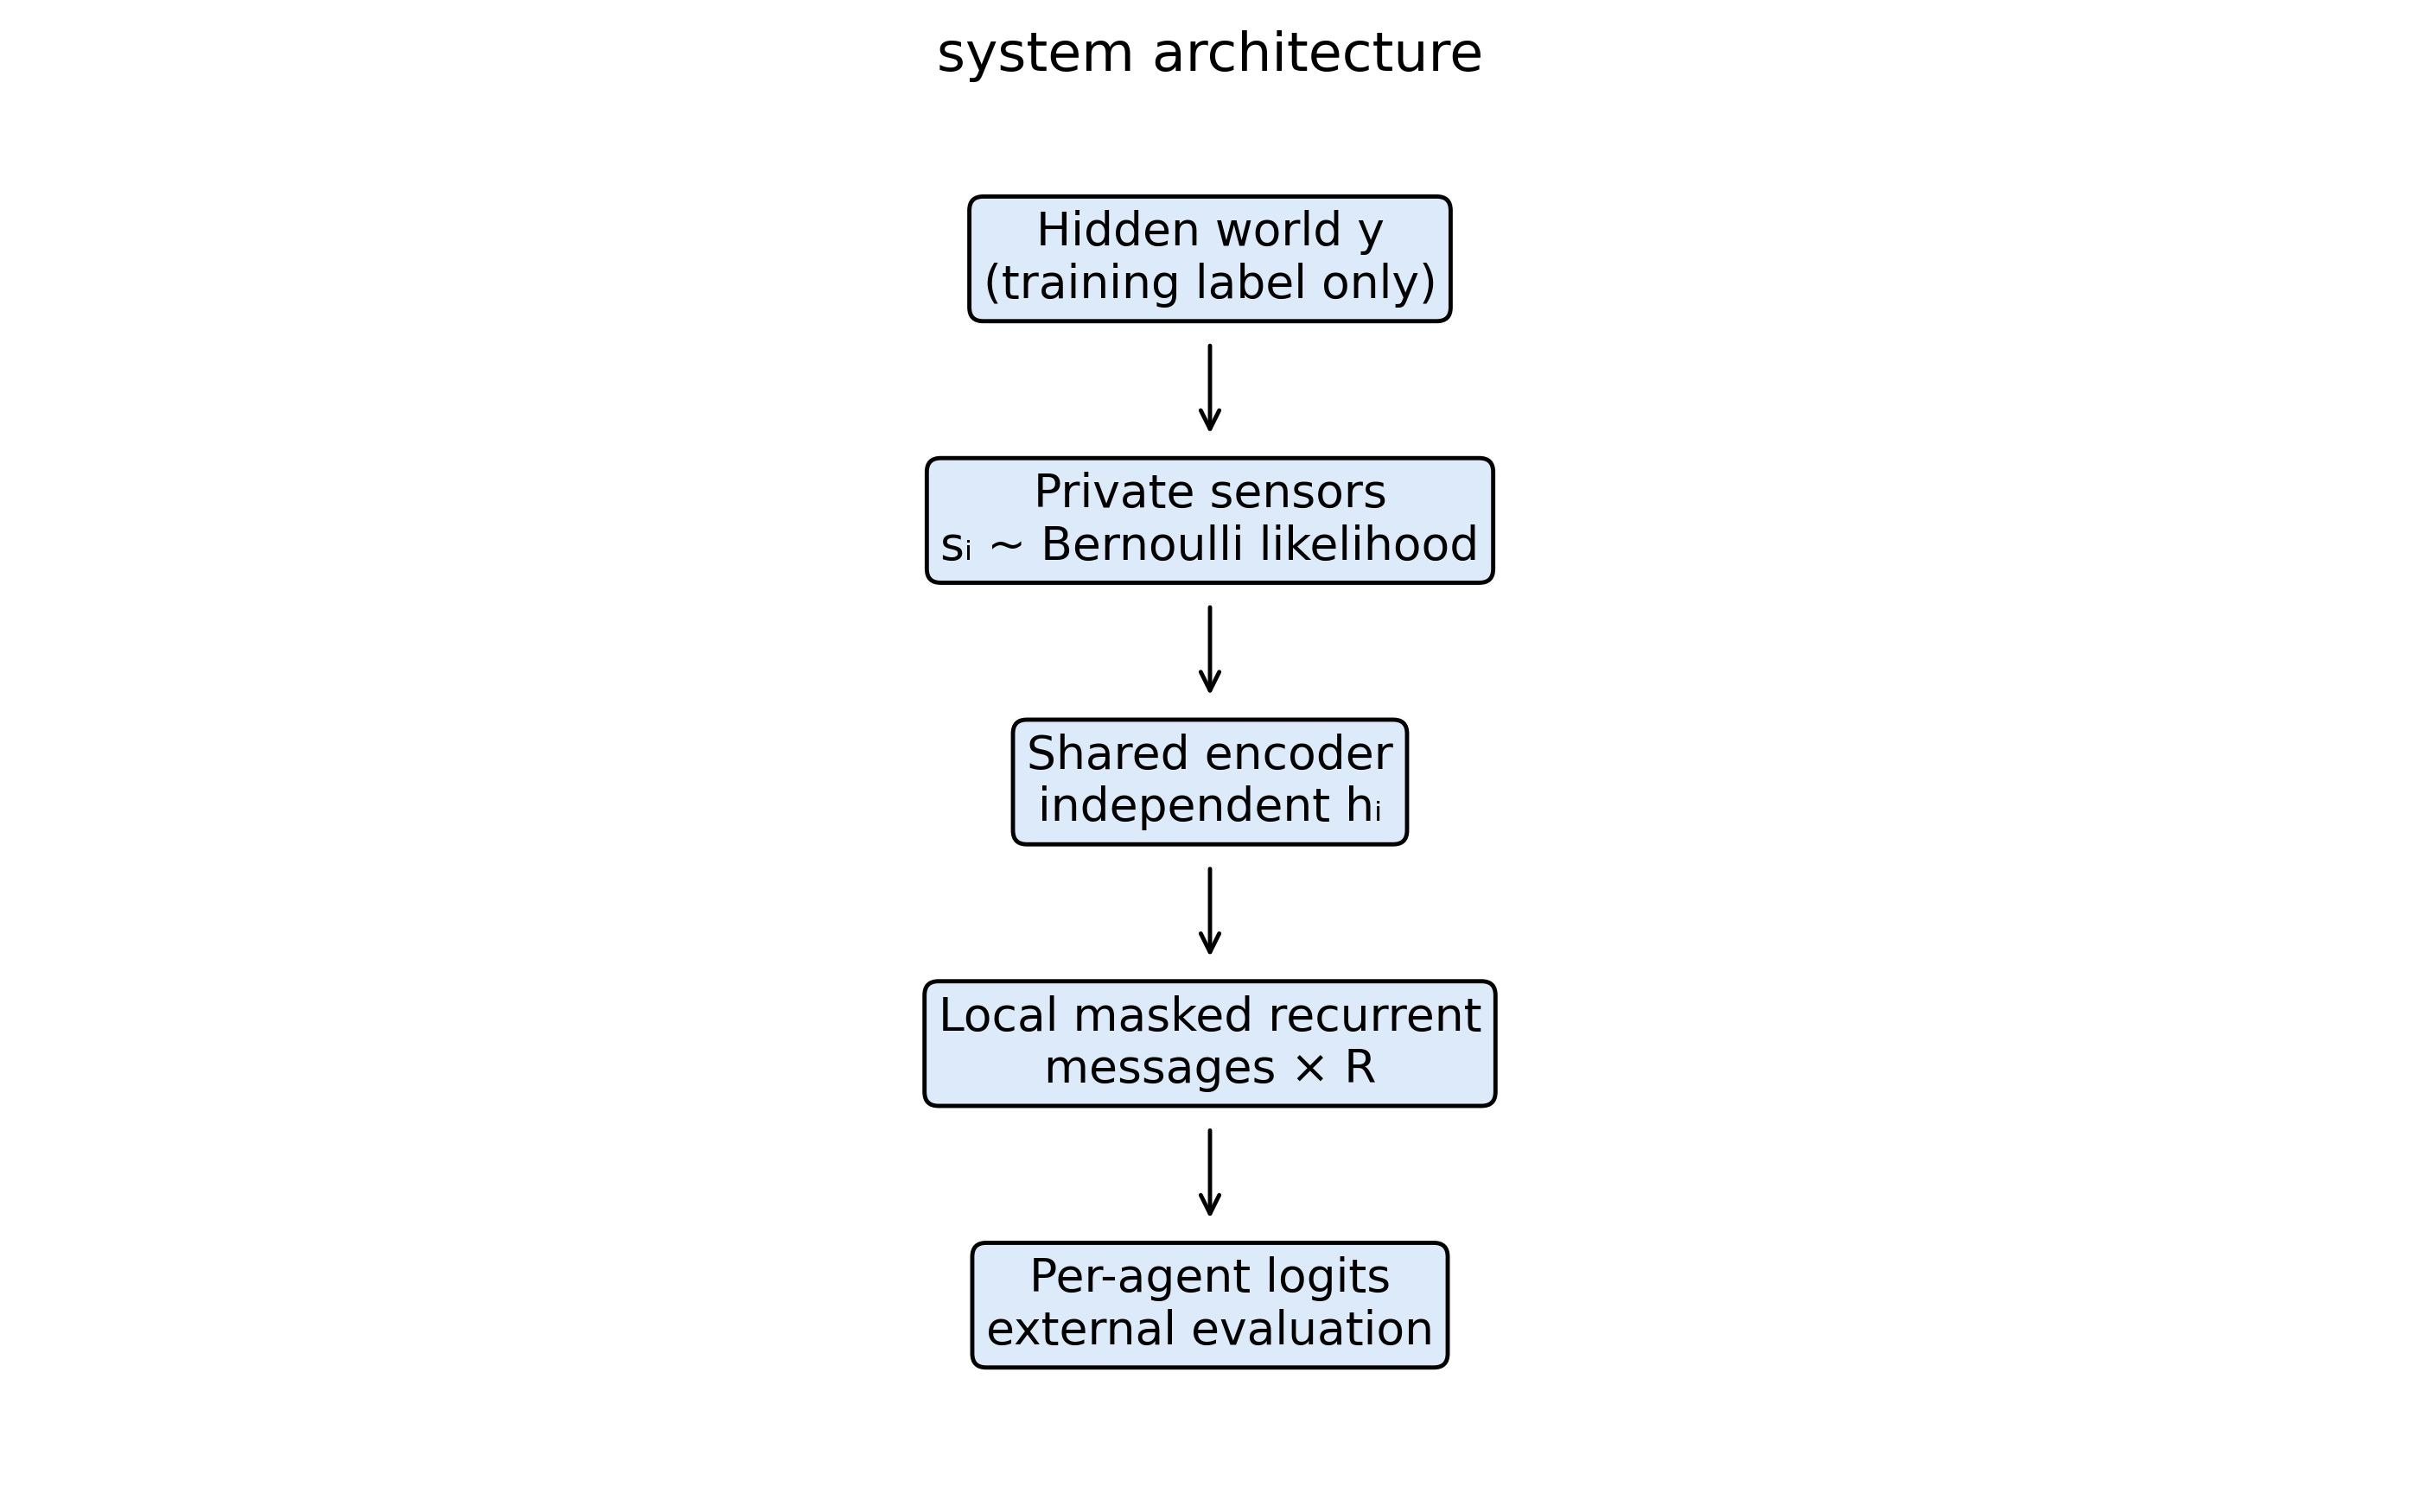
\includegraphics[width=.95\linewidth]{F01_system_architecture.png}}{\fbox{Figure pending completed experiment}}
\caption{System architecture. Architecture schematic; no quantitative results.}
\end{figure}
\begin{figure}[htbp]
\centering
\IfFileExists{../results/figures/F02_agent_communication_graph.png}{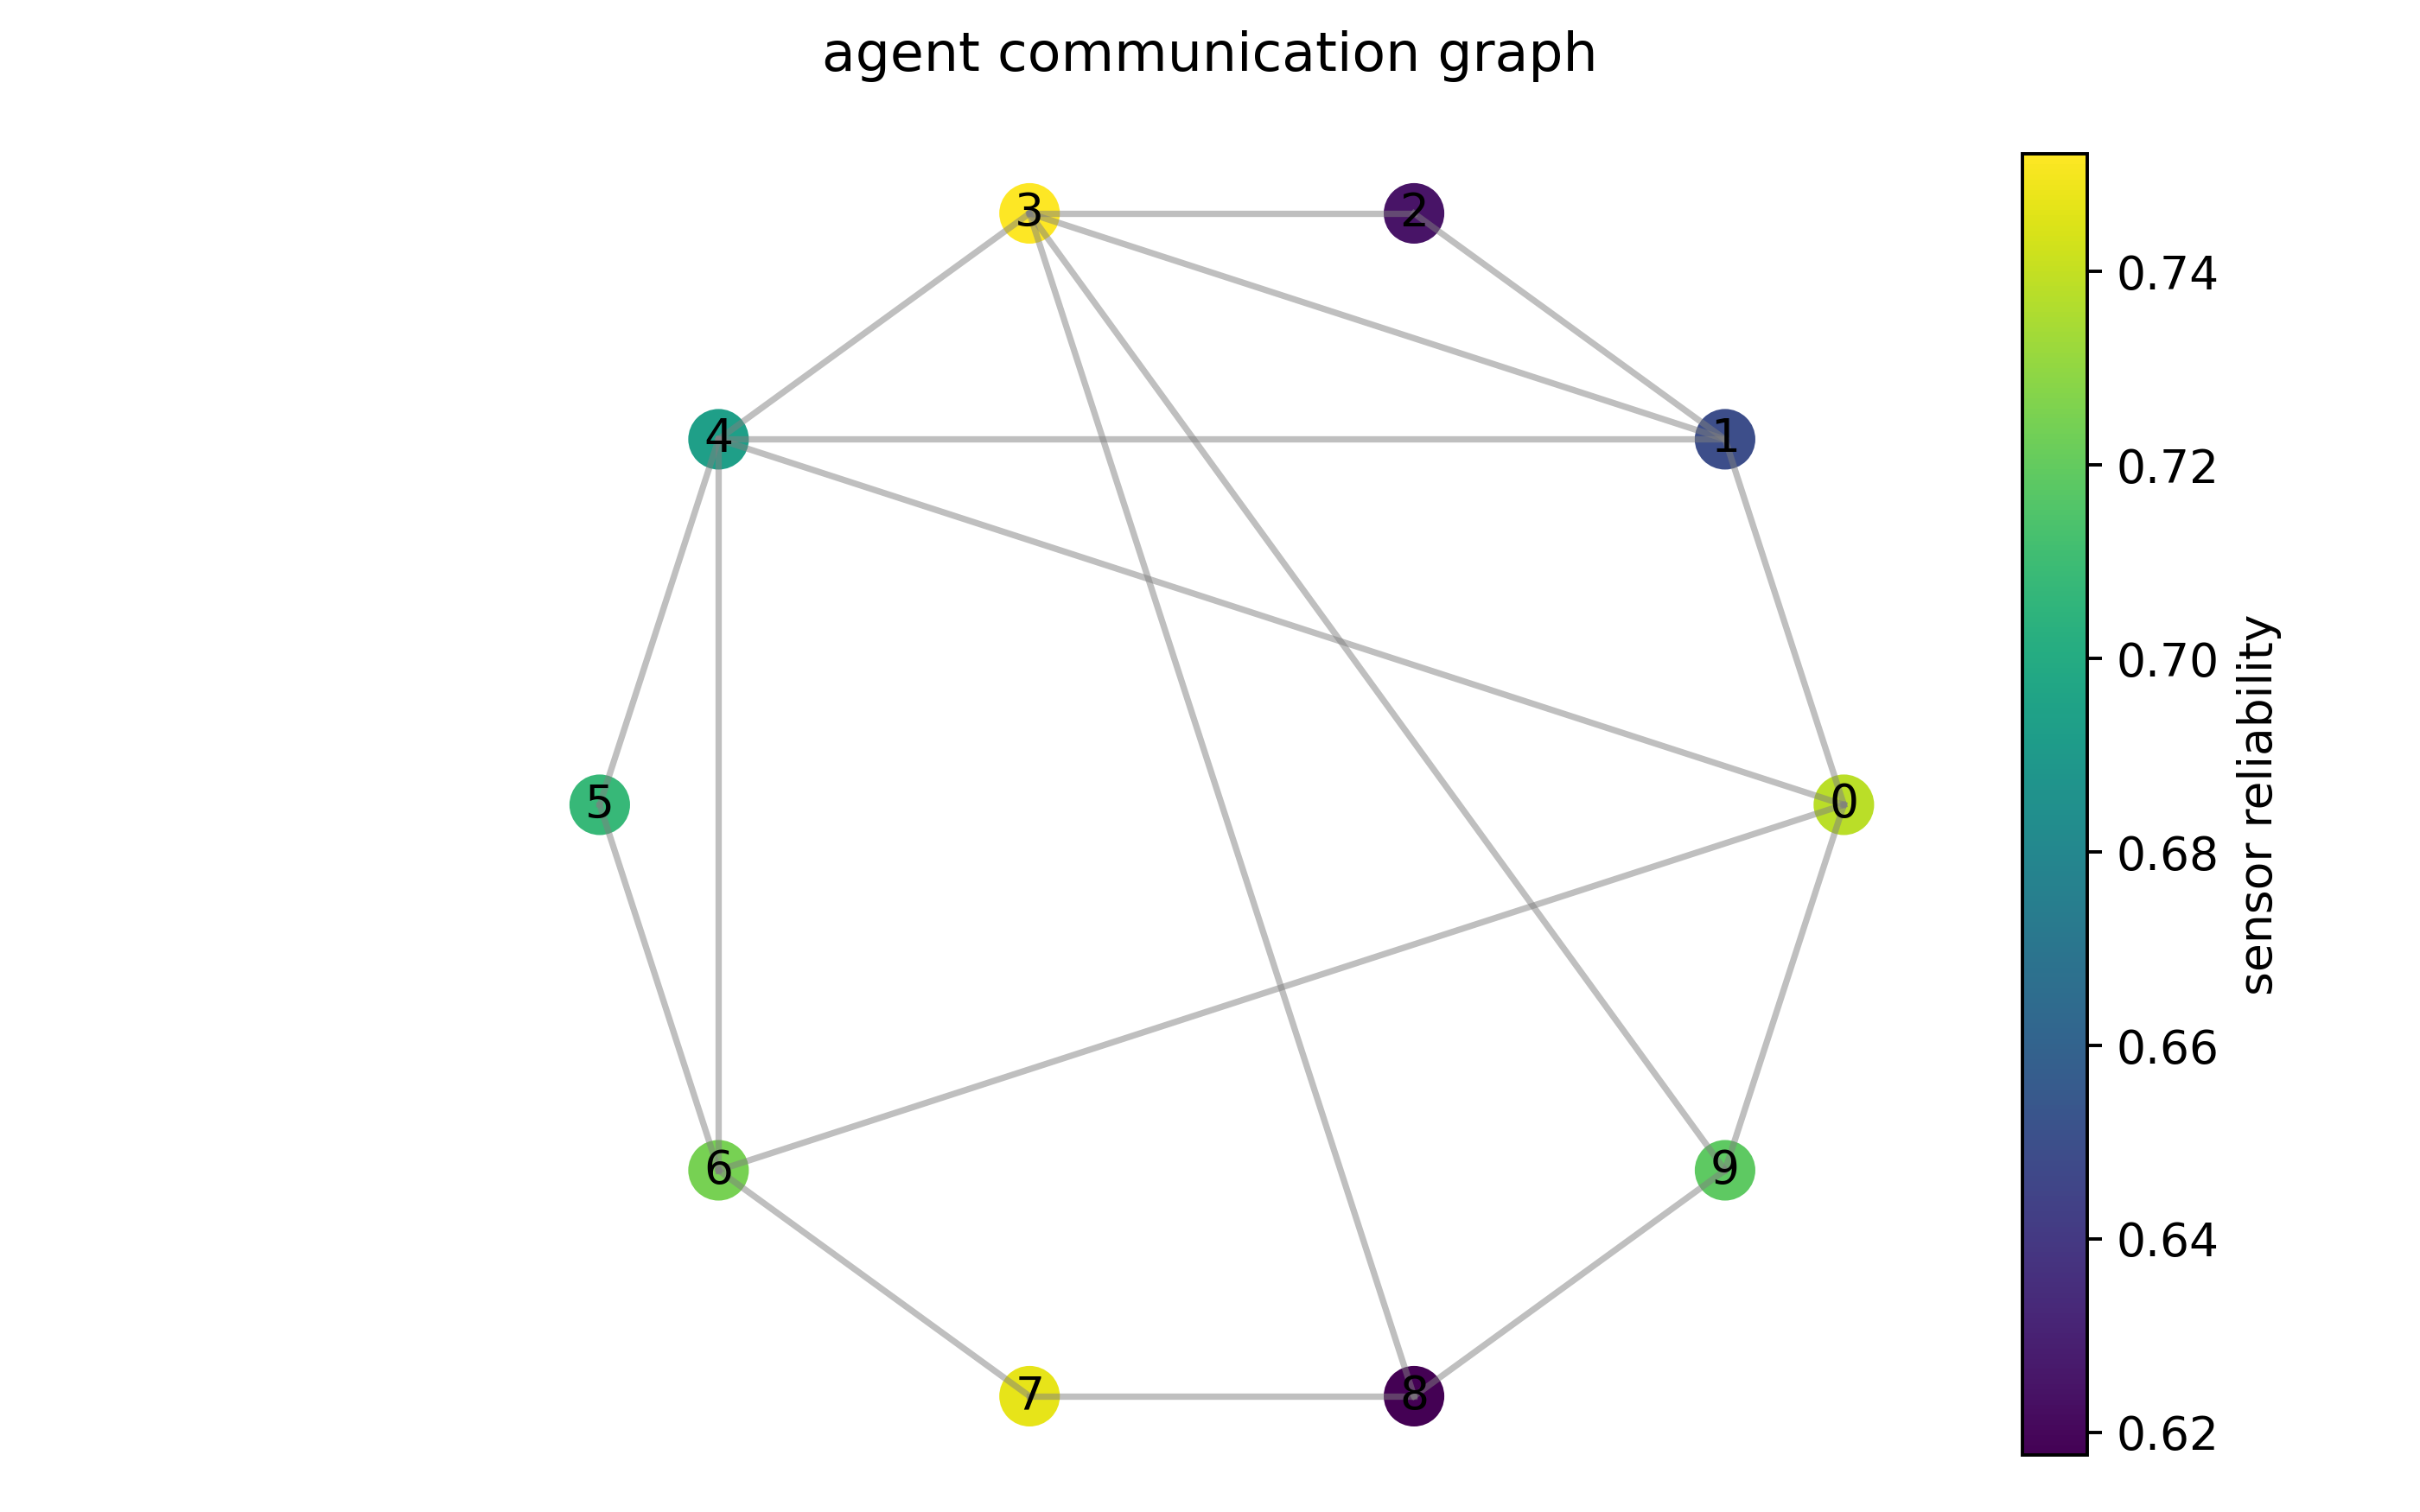
\includegraphics[width=.95\linewidth]{F02_agent_communication_graph.png}}{\fbox{Figure pending completed experiment}}
\caption{Agent communication graph. Generated from saved experimental data; confidence bands, where shown, use training seeds.}
\end{figure}
\begin{figure}[htbp]
\centering
\IfFileExists{../results/figures/F03_consensus_emergence.png}{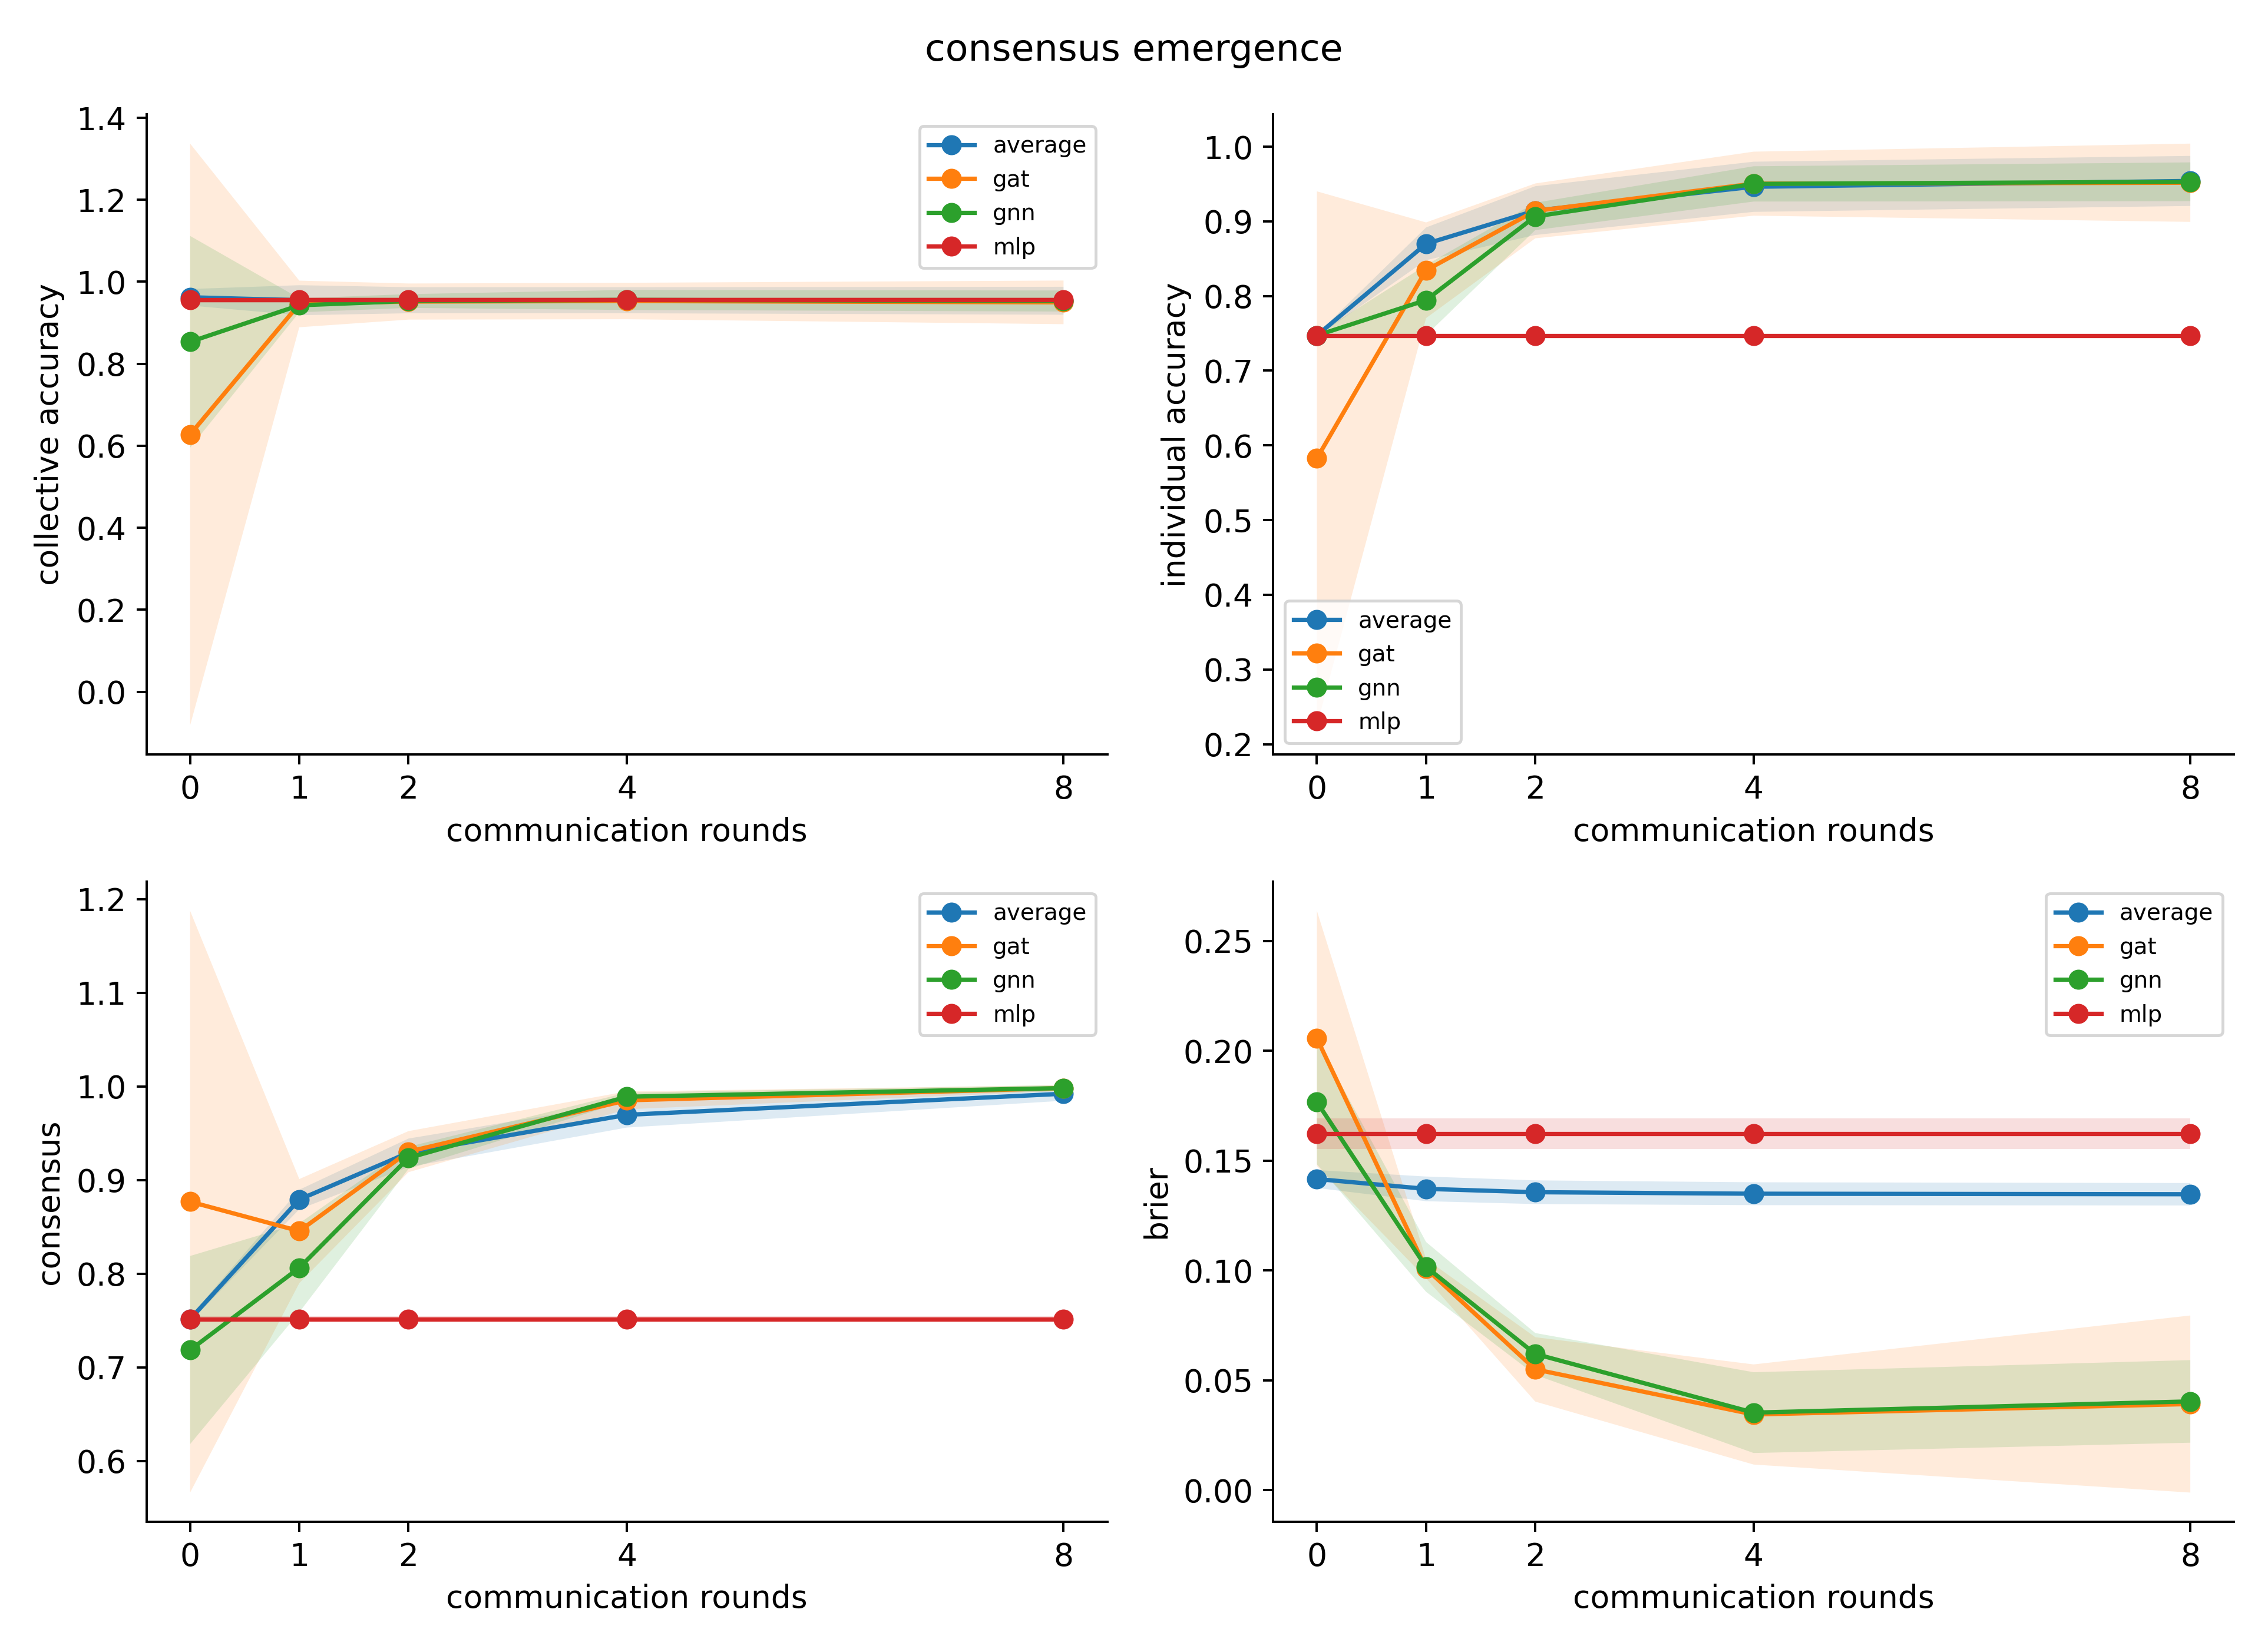
\includegraphics[width=.95\linewidth]{F03_consensus_emergence.png}}{\fbox{Figure pending completed experiment}}
\caption{Consensus emergence. Generated from saved experimental data; confidence bands, where shown, use training seeds.}
\end{figure}
\begin{figure}[htbp]
\centering
\IfFileExists{../results/figures/F04_causal_agent_influence.png}{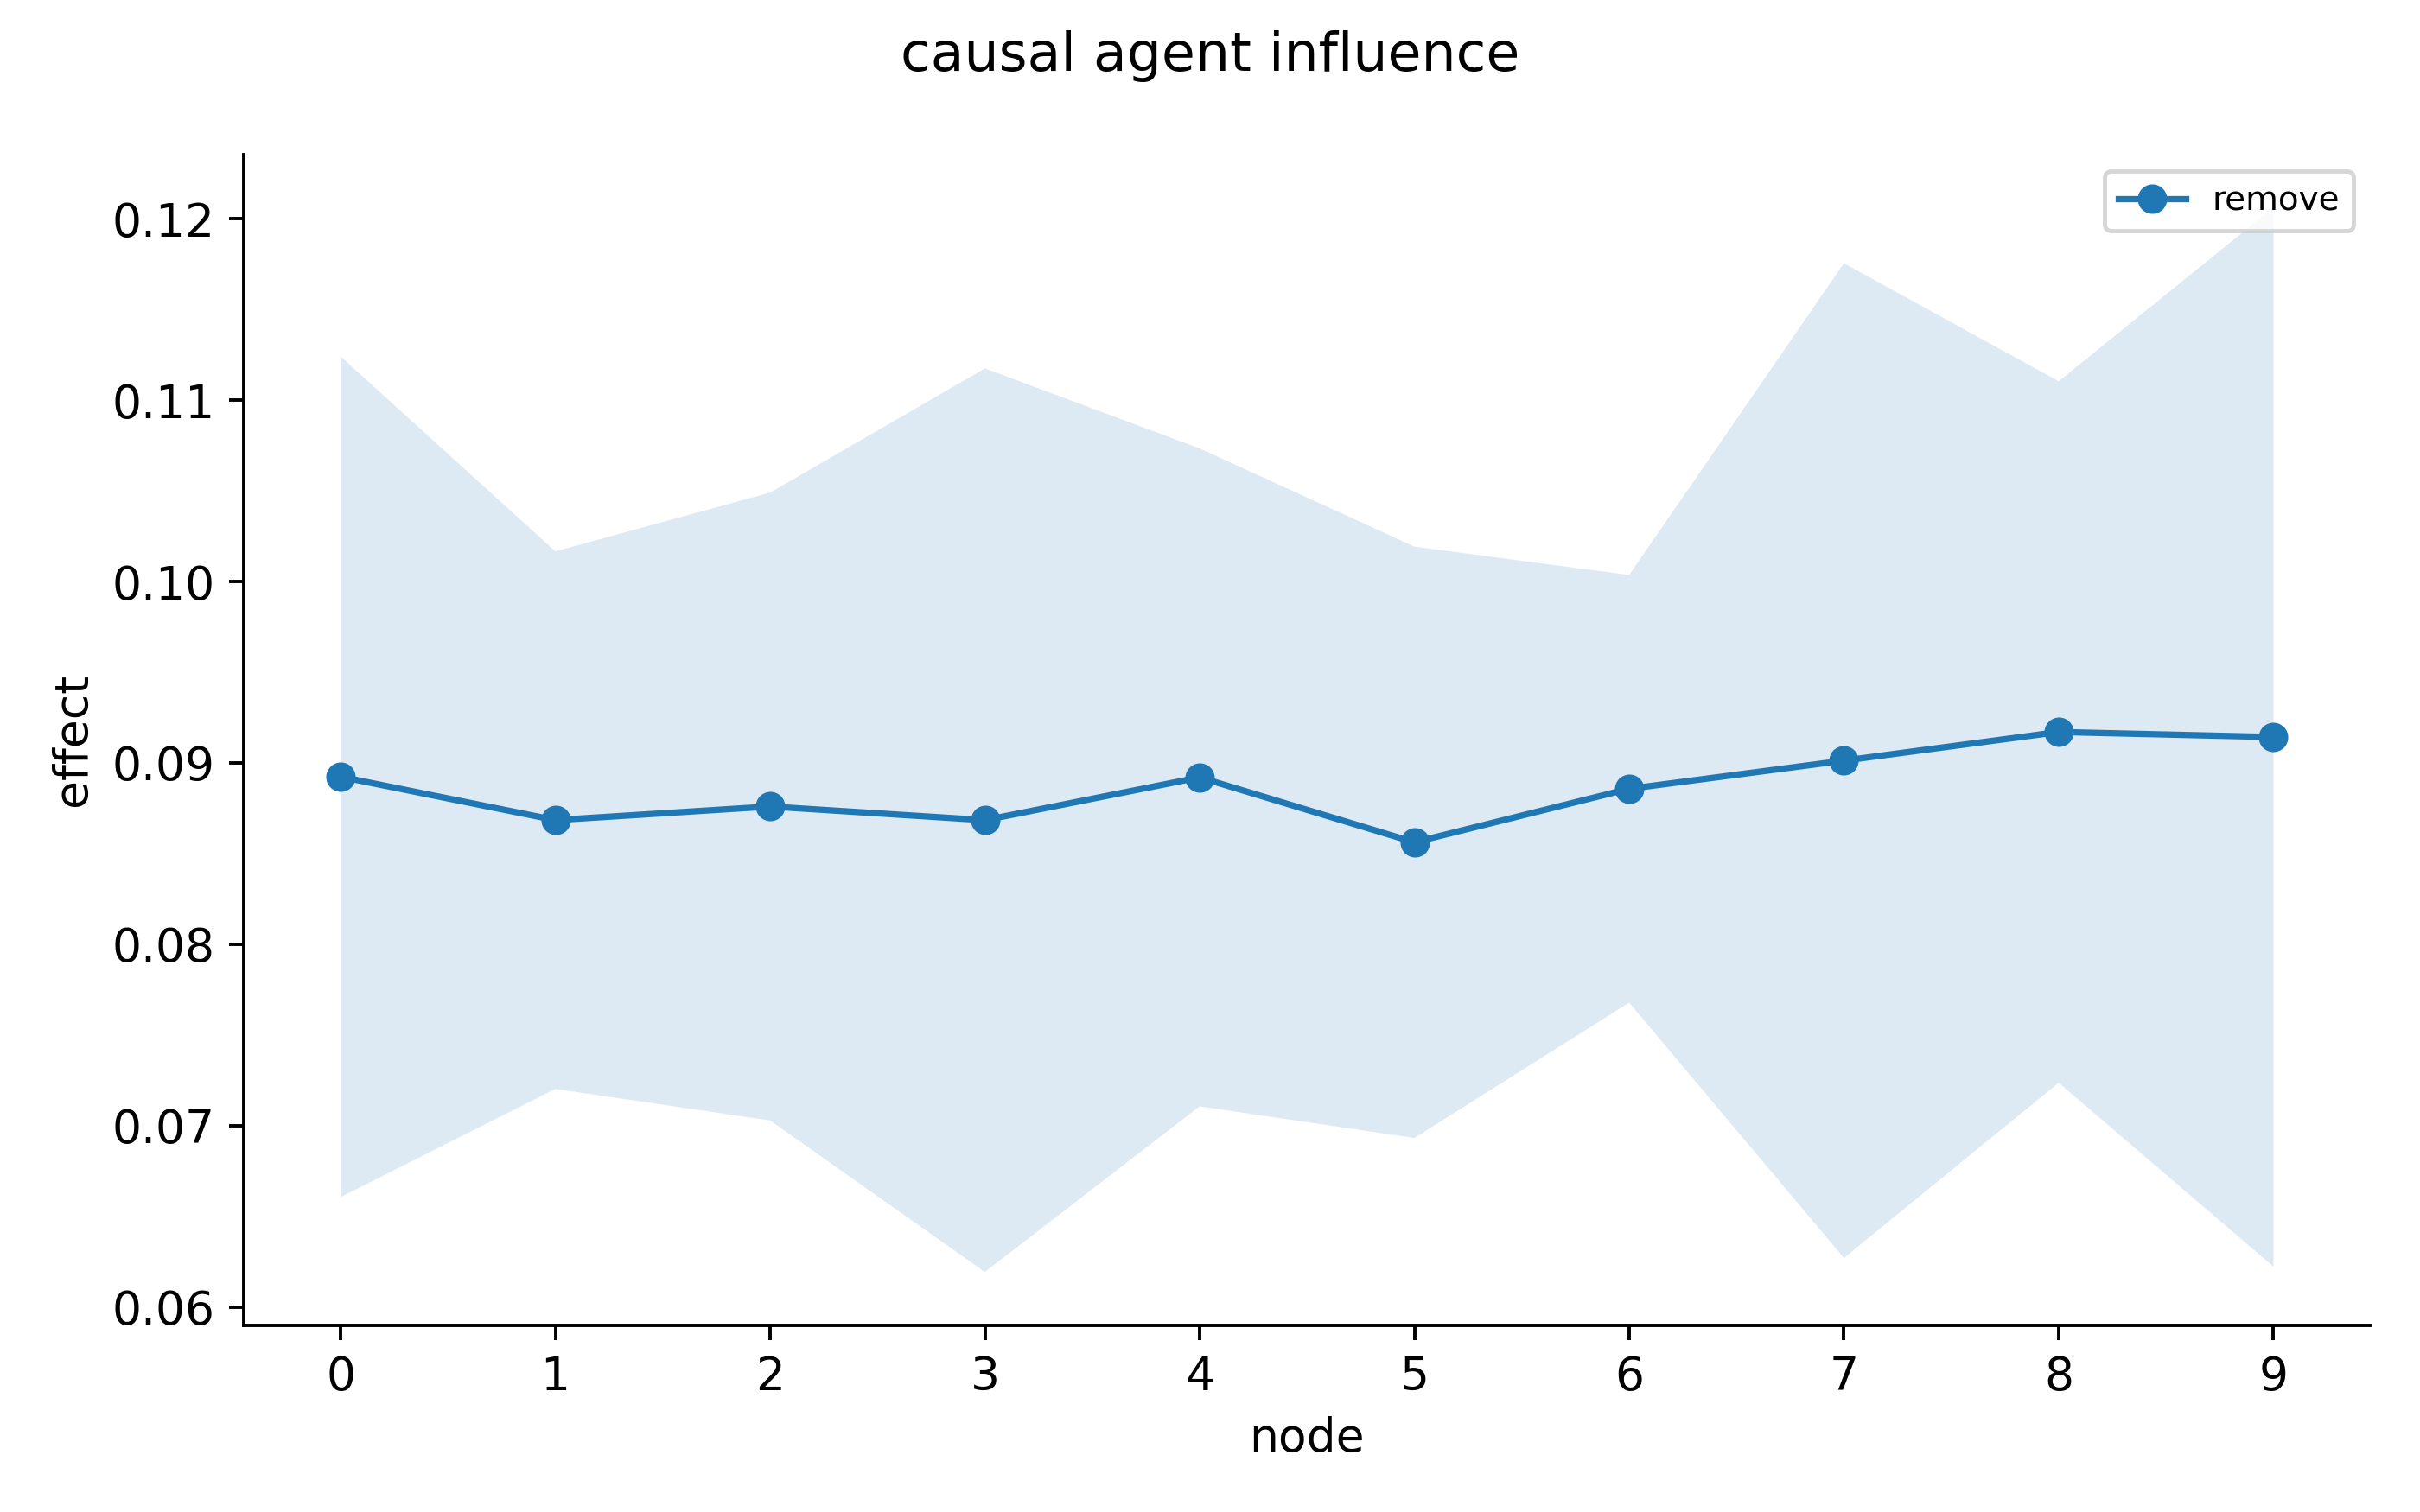
\includegraphics[width=.95\linewidth]{F04_causal_agent_influence.png}}{\fbox{Figure pending completed experiment}}
\caption{Causal agent influence. Generated from saved experimental data; confidence bands, where shown, use training seeds.}
\end{figure}
\begin{figure}[htbp]
\centering
\IfFileExists{../results/figures/F05_communication_circuit_map.png}{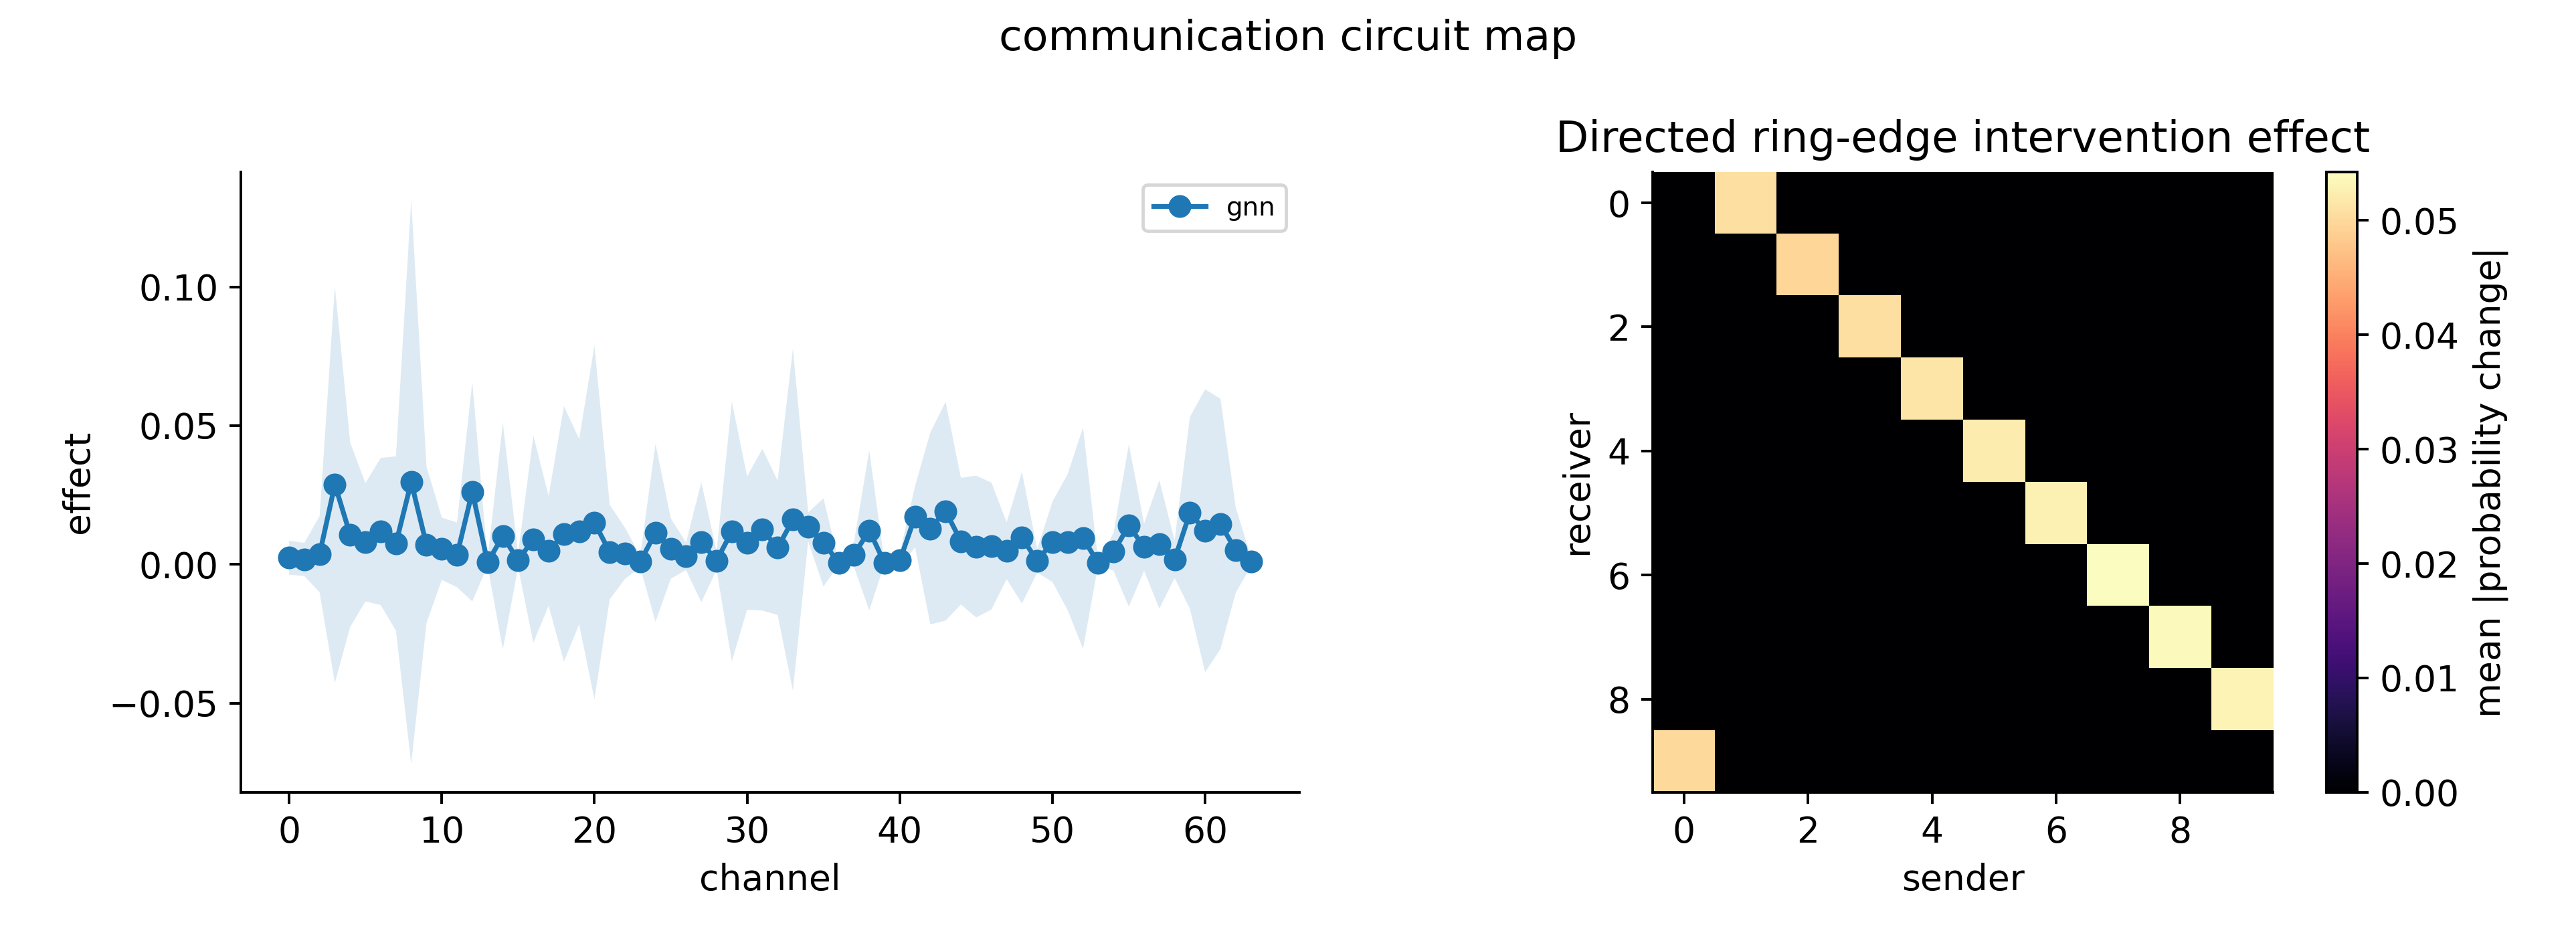
\includegraphics[width=.95\linewidth]{F05_communication_circuit_map.png}}{\fbox{Figure pending completed experiment}}
\caption{Communication circuit map. Generated from saved experimental data; confidence bands, where shown, use training seeds.}
\end{figure}
\begin{figure}[htbp]
\centering
\IfFileExists{../results/figures/F06_neural_representation_heatmap.png}{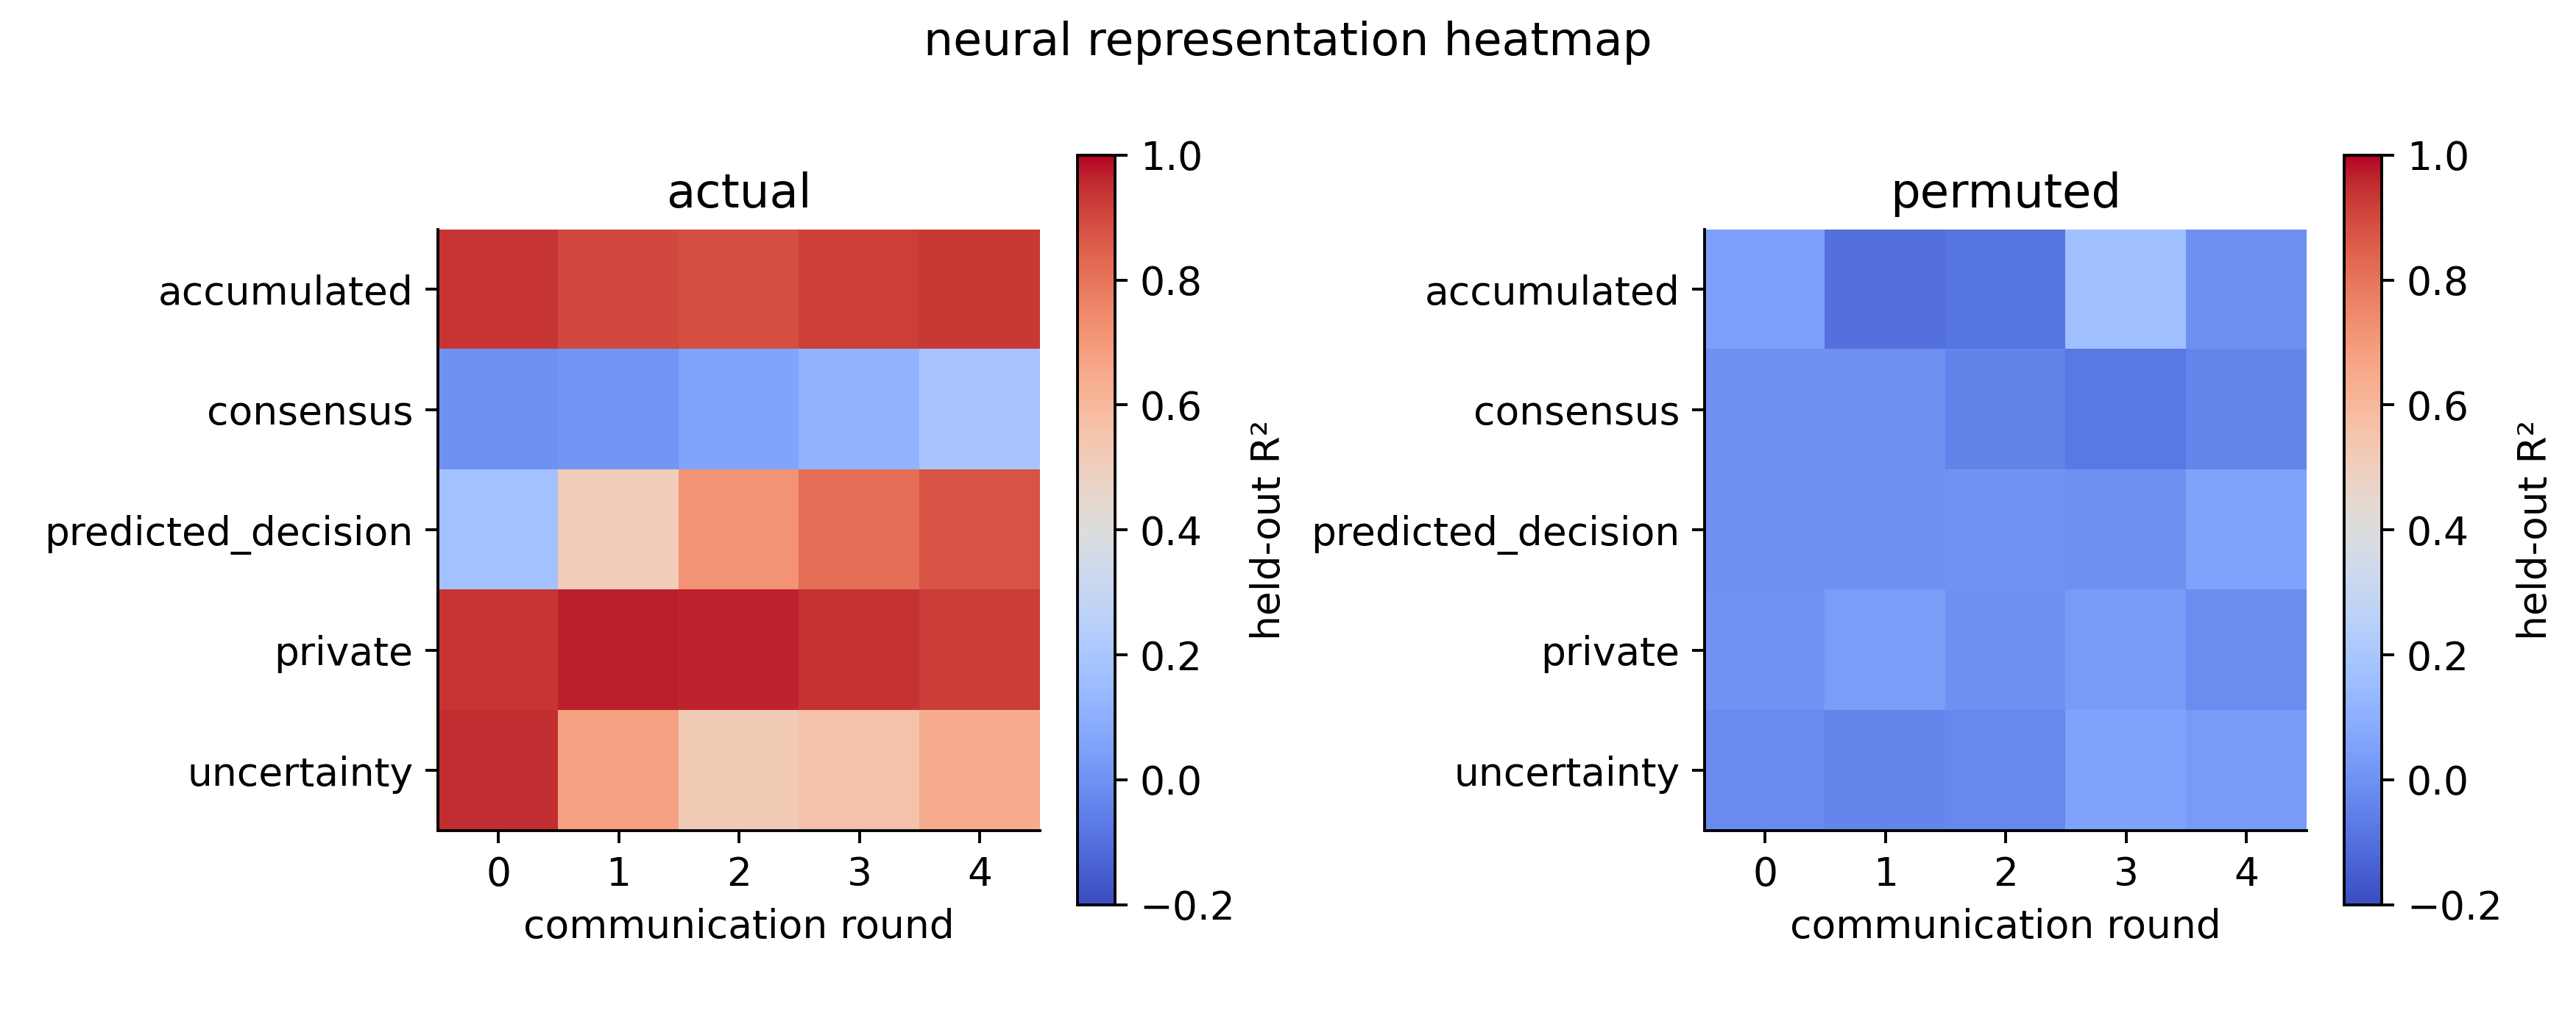
\includegraphics[width=.95\linewidth]{F06_neural_representation_heatmap.png}}{\fbox{Figure pending completed experiment}}
\caption{Neural representation heatmap. Generated from saved experimental data; confidence bands, where shown, use training seeds.}
\end{figure}
\begin{figure}[htbp]
\centering
\IfFileExists{../results/figures/F07_targeted_ablation.png}{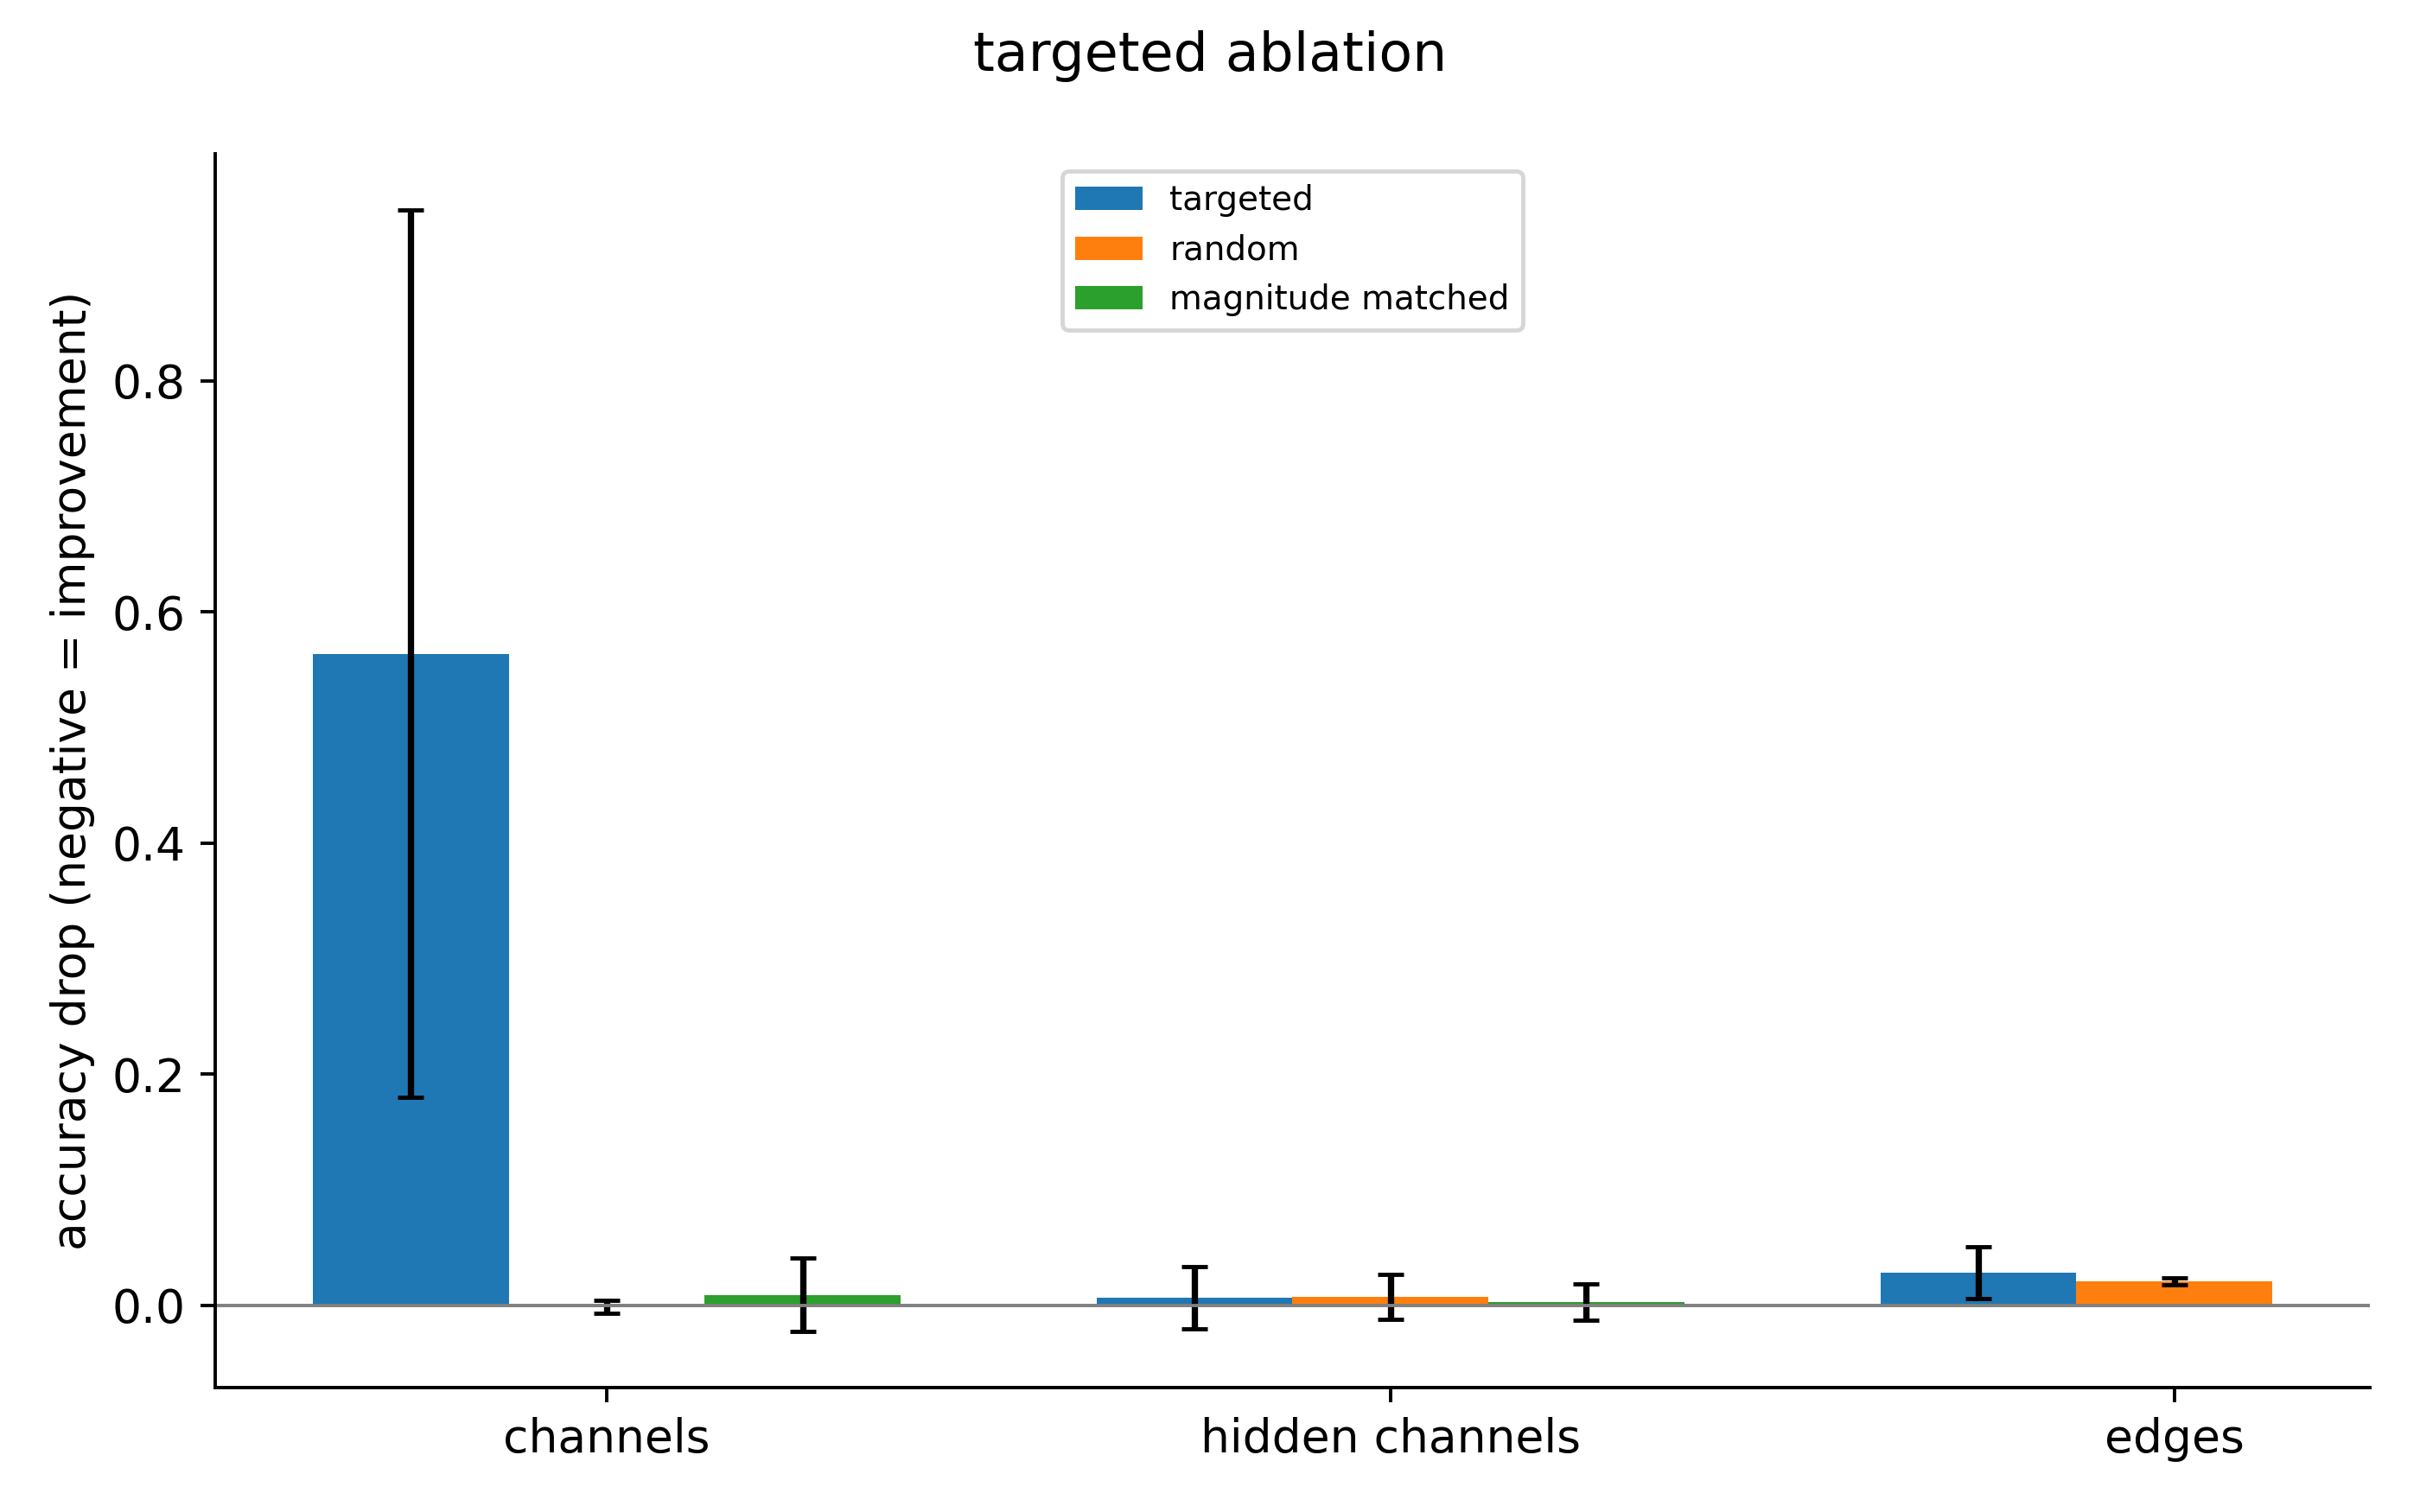
\includegraphics[width=.95\linewidth]{F07_targeted_ablation.png}}{\fbox{Figure pending completed experiment}}
\caption{Targeted ablation. Generated from saved experimental data; confidence bands, where shown, use training seeds.}
\end{figure}
\begin{figure}[htbp]
\centering
\IfFileExists{../results/figures/F08_activation_patching_recovery.png}{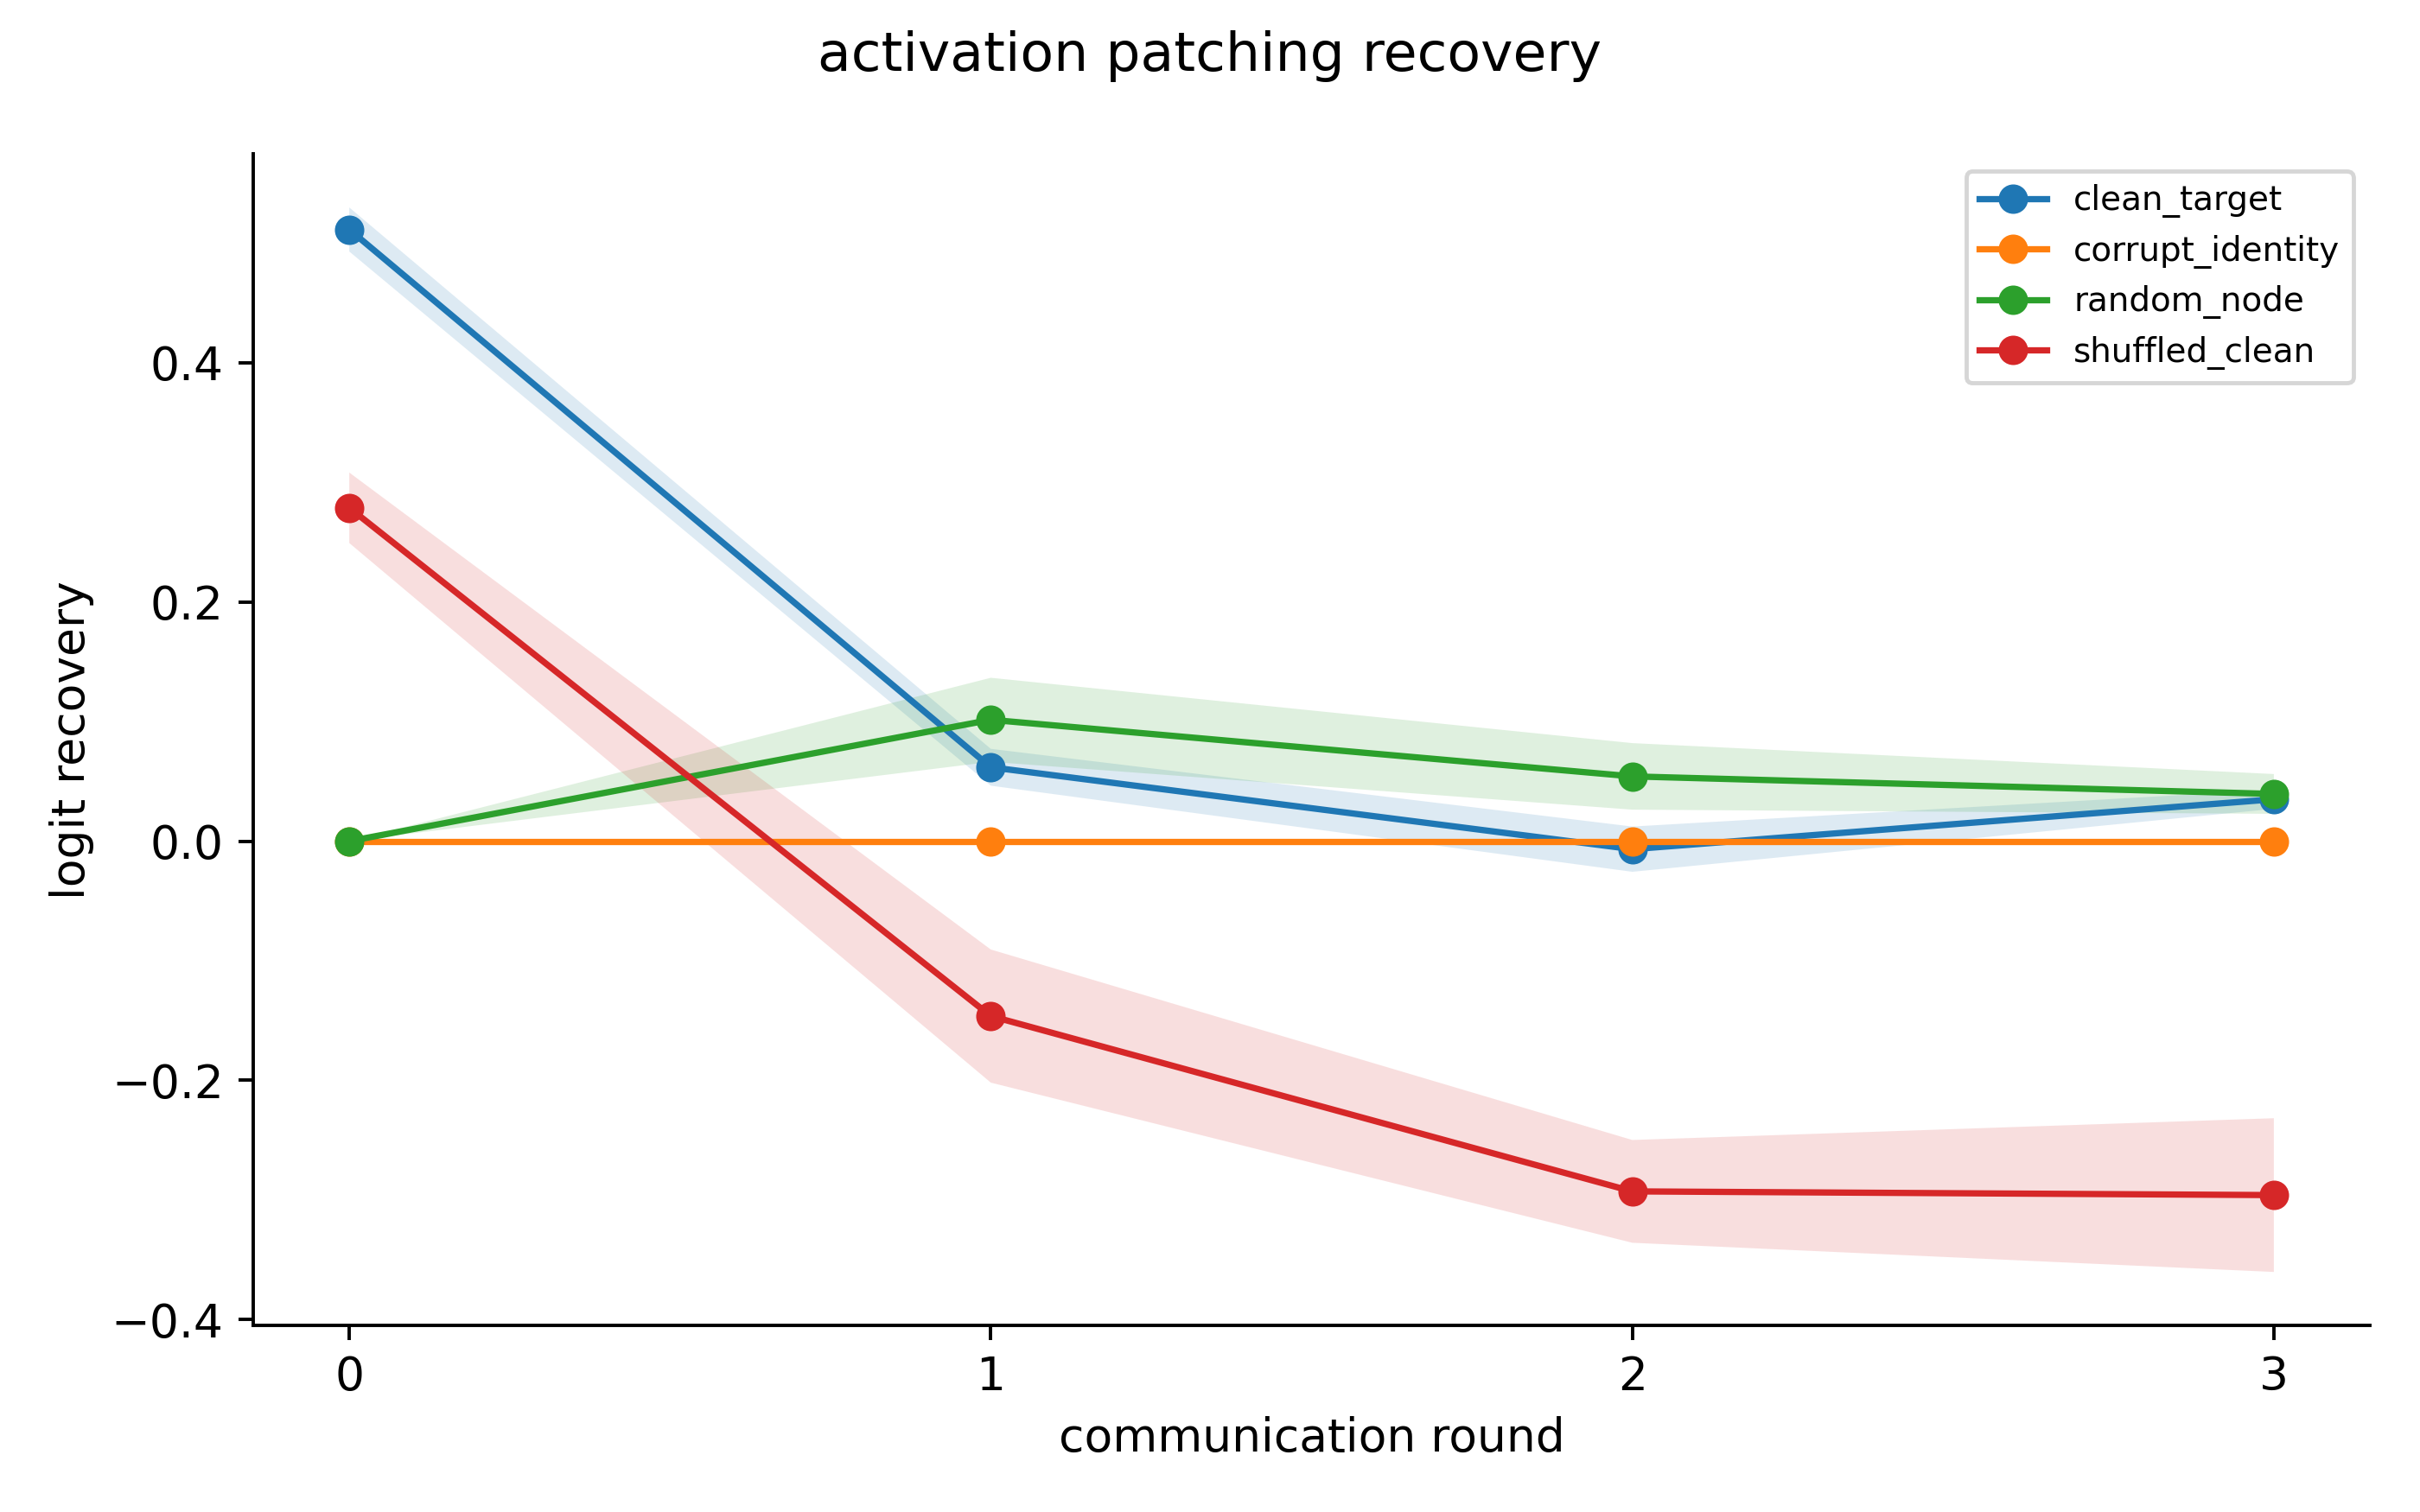
\includegraphics[width=.95\linewidth]{F08_activation_patching_recovery.png}}{\fbox{Figure pending completed experiment}}
\caption{Activation patching recovery. Generated from saved experimental data; confidence bands, where shown, use training seeds.}
\end{figure}
\begin{figure}[htbp]
\centering
\IfFileExists{../results/figures/F09_failure_robustness.png}{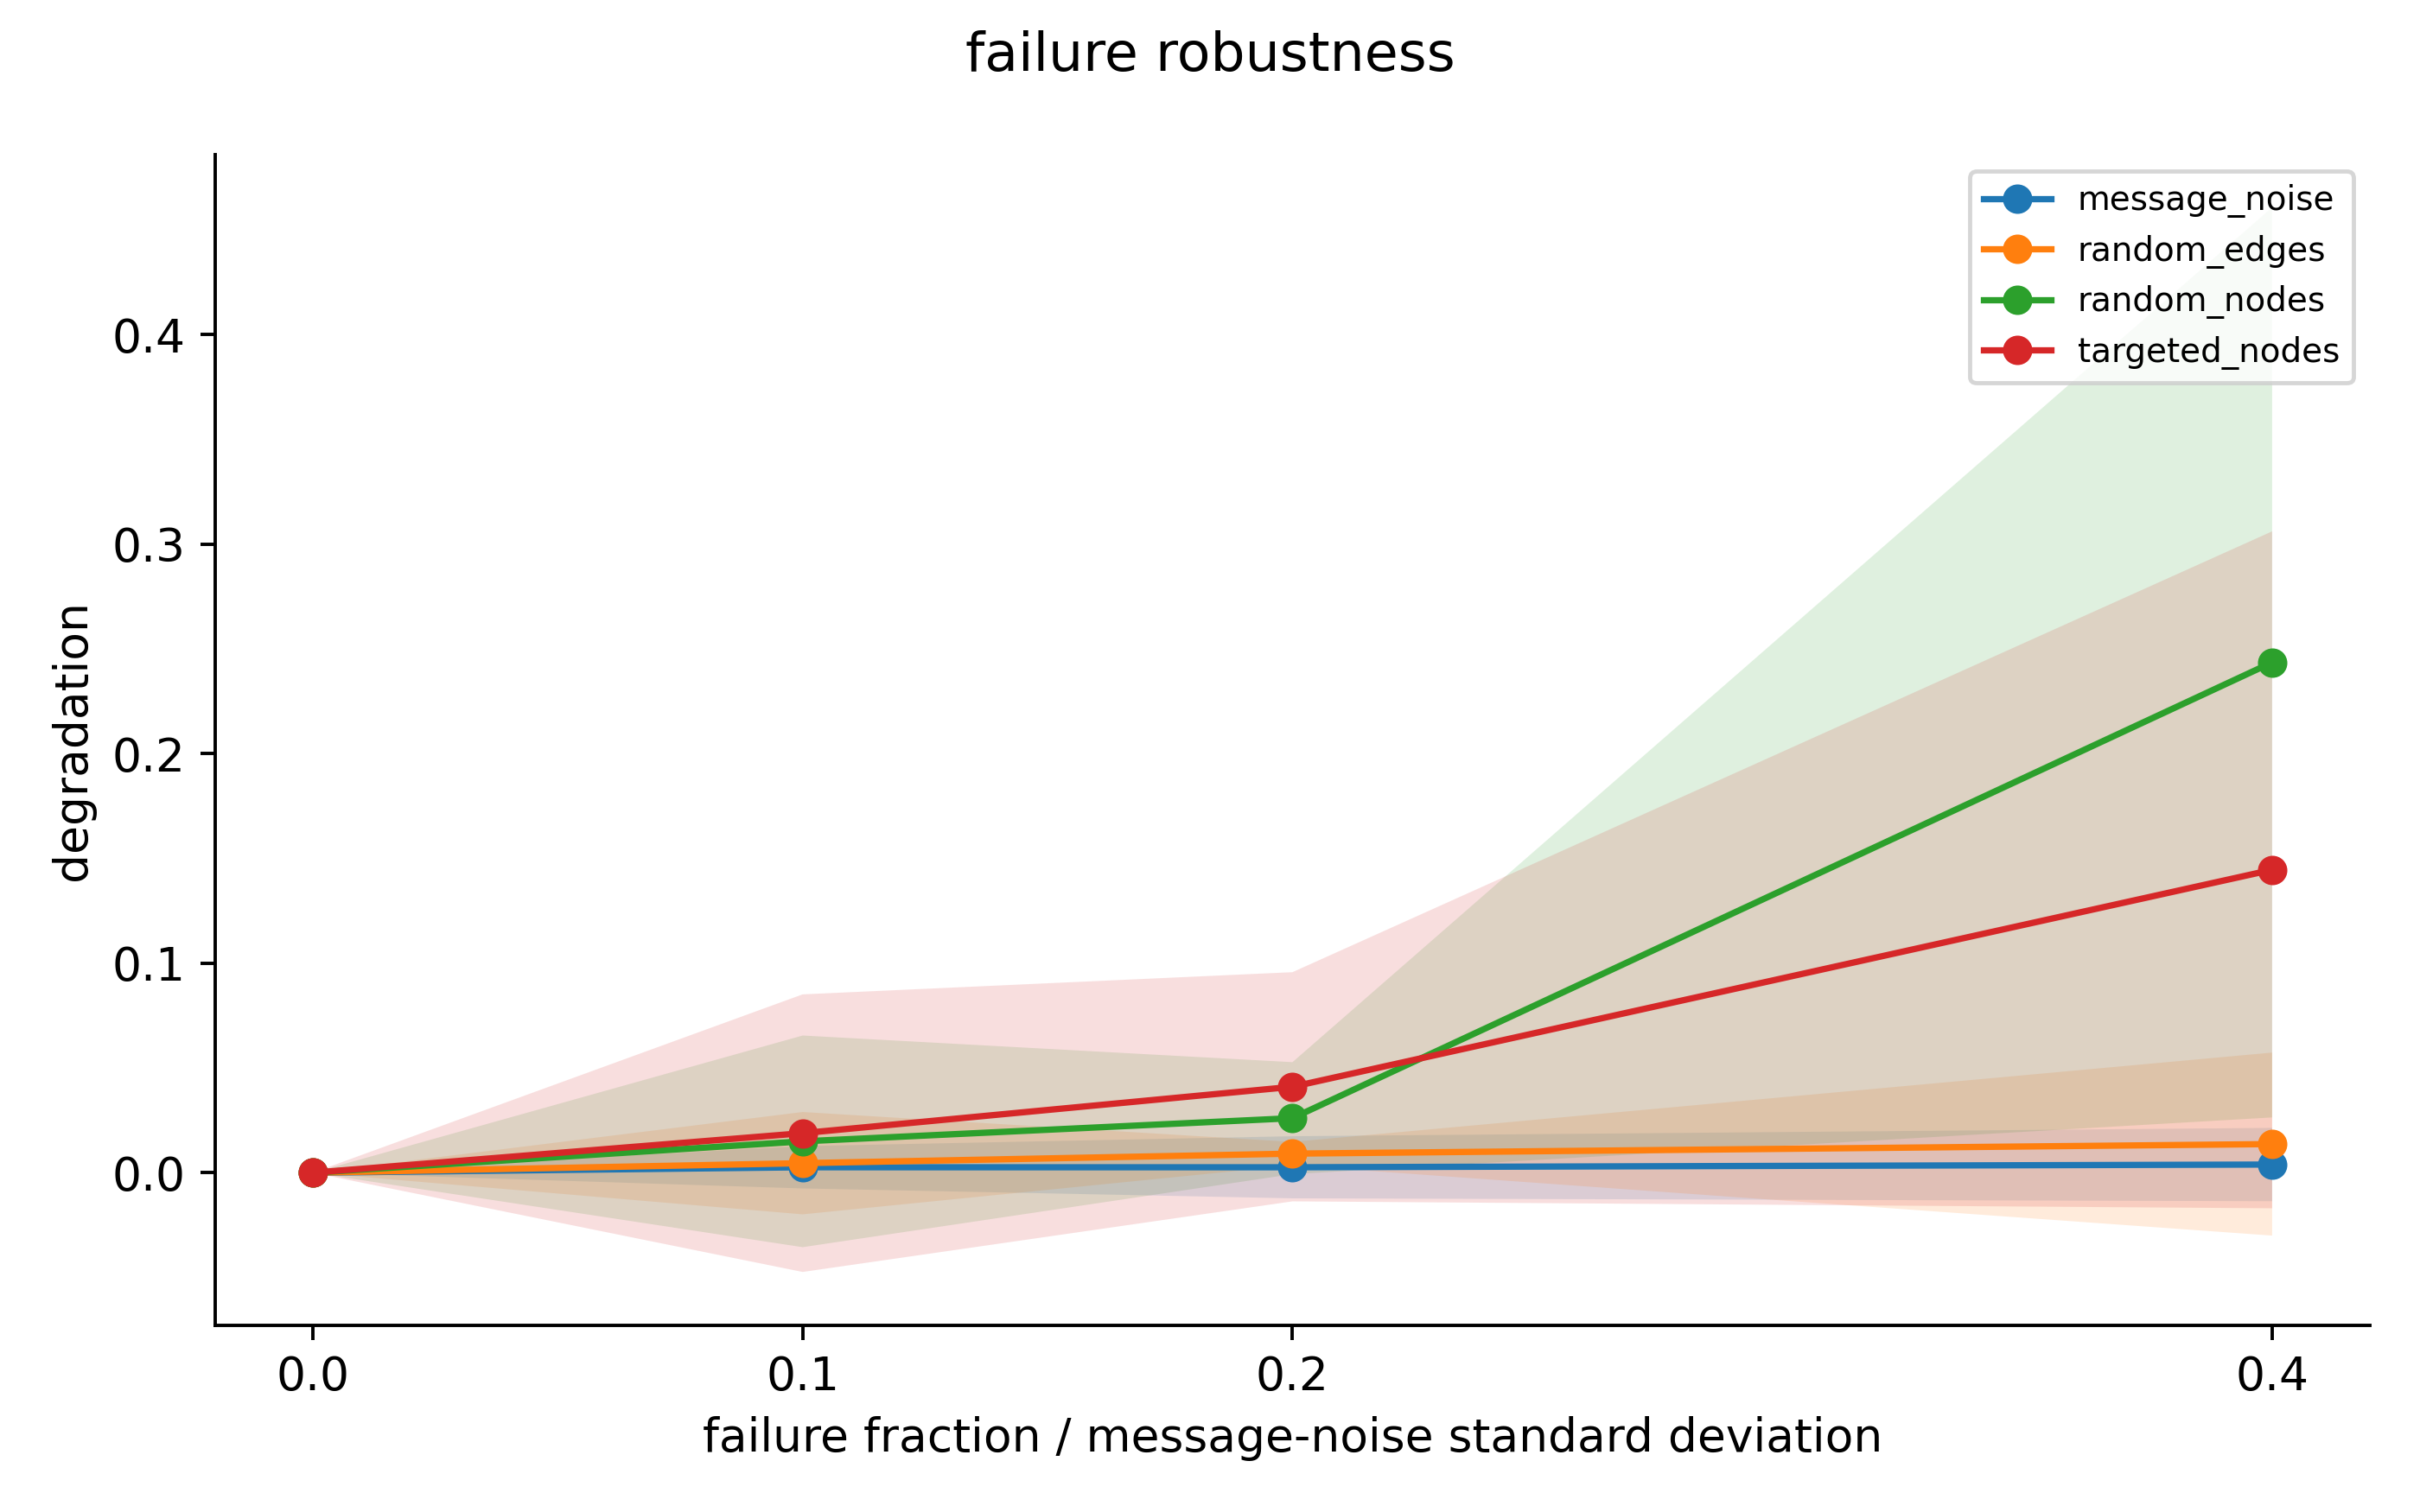
\includegraphics[width=.95\linewidth]{F09_failure_robustness.png}}{\fbox{Figure pending completed experiment}}
\caption{Failure robustness. Generated from saved experimental data; confidence bands, where shown, use training seeds.}
\end{figure}
\begin{figure}[htbp]
\centering
\IfFileExists{../results/figures/F10_swarm_size_generalization.png}{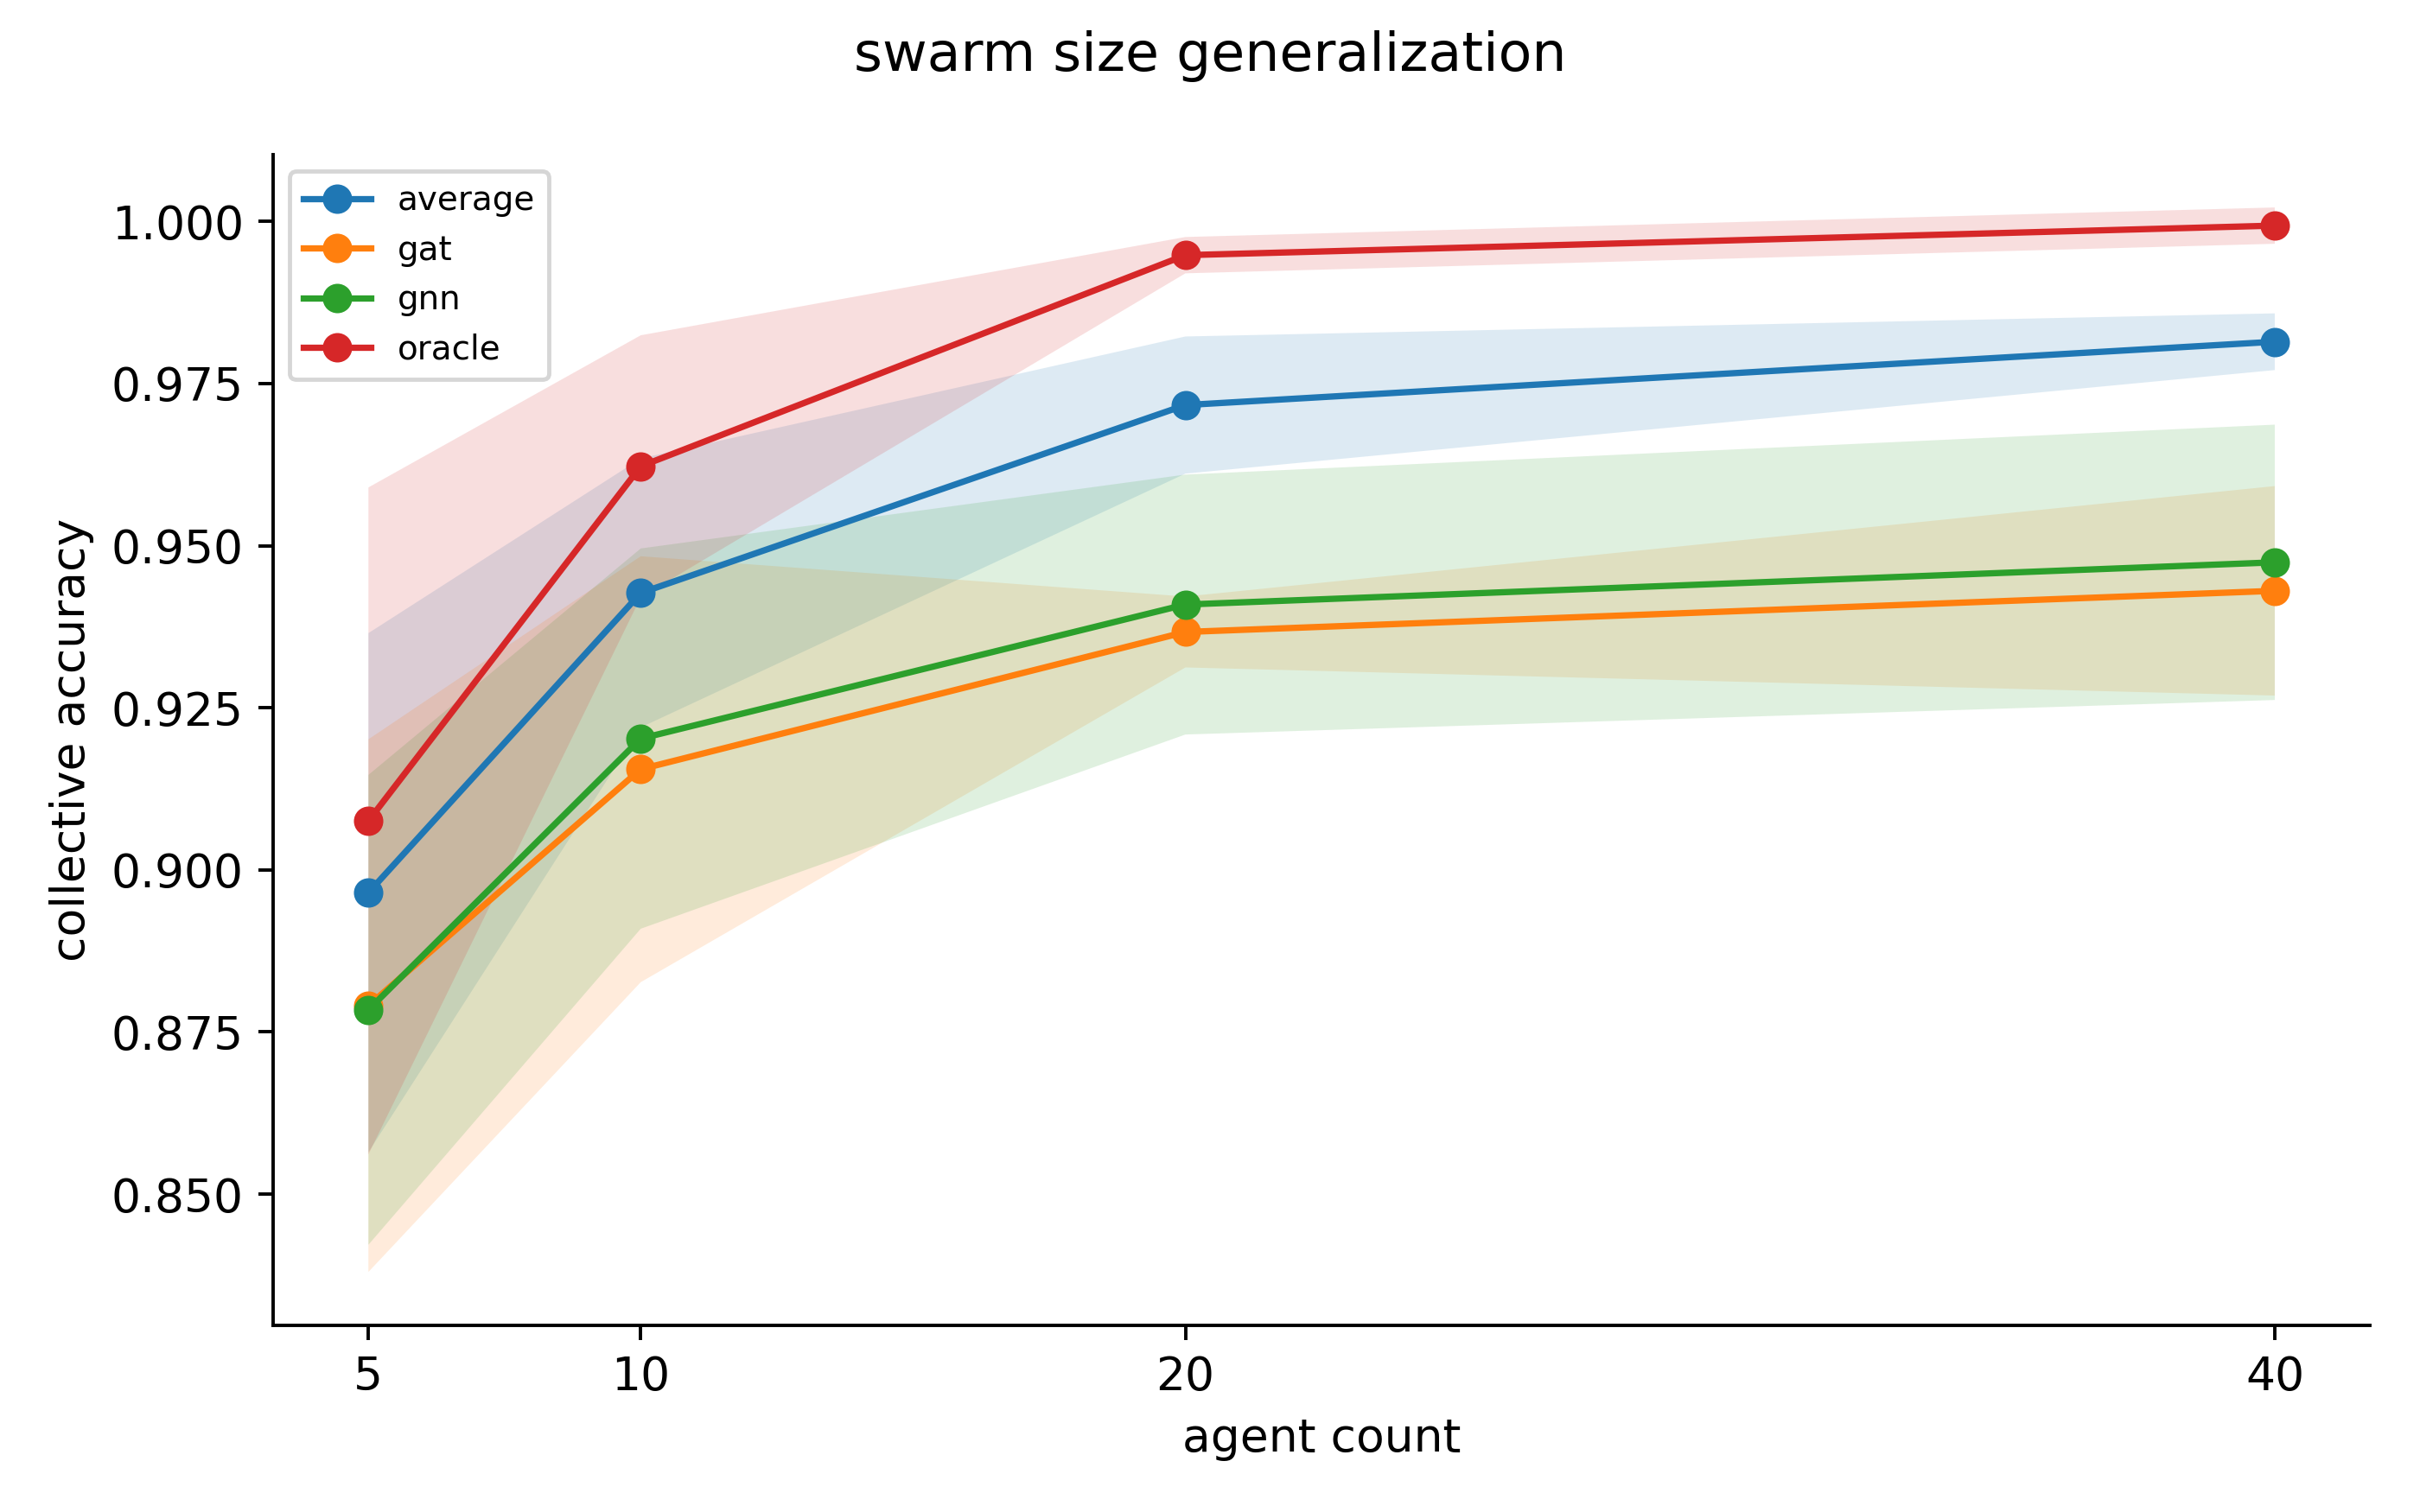
\includegraphics[width=.95\linewidth]{F10_swarm_size_generalization.png}}{\fbox{Figure pending completed experiment}}
\caption{Swarm size generalization. Generated from saved experimental data; confidence bands, where shown, use training seeds.}
\end{figure}
\clearpage
\begin{thebibliography}{9}
\bibitem{gilmer} J. Gilmer, S. S. Schoenholz, P. F. Riley, O. Vinyals, and G. E. Dahl. Neural Message Passing for Quantum Chemistry. 2017. \url{https://arxiv.org/abs/1704.01212}.
\bibitem{gat} P. Veličković, G. Cucurull, A. Casanova, A. Romero, P. Liò, and Y. Bengio. Graph Attention Networks. 2017. \url{https://arxiv.org/abs/1710.10903}.
\bibitem{meng} K. Meng, D. Bau, A. Andonian, and Y. Belinkov. Locating and Editing Factual Associations in GPT. 2022. \url{https://arxiv.org/abs/2202.05262}.
\bibitem{belinkov} Y. Belinkov. Probing Classifiers: Promises, Shortcomings, and Advances. 2021 preprint. \url{https://arxiv.org/abs/2102.12452}.
\end{thebibliography}
\end{document}
